% FC format (LNCS / llncs.cls)
\documentclass[runningheads]{llncs}

\usepackage[T1]{fontenc}
\usepackage{graphicx}
\usepackage{url}
\usepackage{cryptocode}
\usepackage{algorithm}
\usepackage{algpseudocode}
\usepackage{amsmath}
\usepackage{enumitem}
\usepackage{amssymb}
\usepackage{subfig}
\usepackage{booktabs}
\usepackage{adjustbox}
\usepackage{xspace}
\usepackage{multirow}
\usepackage{float}
\usepackage{pgfplots}
\pgfplotsset{compat=1.18}

% Color gradient definitions for multi-spec figures
% Fig 5: Red gradient (Naive) / Blue gradient (Freivalds)
\definecolor{redspec1}{RGB}{240, 140, 140}
\definecolor{redspec2}{RGB}{220, 90, 90}
\definecolor{redspec3}{RGB}{200, 50, 50}
\definecolor{redspec4}{RGB}{160, 20, 20}
\definecolor{redspec5}{RGB}{110, 0, 0}
\definecolor{bluespec1}{RGB}{120, 170, 240}
\definecolor{bluespec2}{RGB}{80, 130, 210}
\definecolor{bluespec3}{RGB}{50, 100, 190}
\definecolor{bluespec4}{RGB}{25, 60, 150}
\definecolor{bluespec5}{RGB}{0, 25, 100}
% Fig 6: Orange gradient (BERT) / Green gradient (Nystrom)
\definecolor{ornspec1}{RGB}{245, 170, 80}
\definecolor{ornspec2}{RGB}{230, 130, 40}
\definecolor{ornspec3}{RGB}{200, 100, 10}
\definecolor{ornspec4}{RGB}{170, 70, 0}
\definecolor{ornspec5}{RGB}{120, 45, 0}
\definecolor{grnspec1}{RGB}{100, 190, 120}
\definecolor{grnspec2}{RGB}{50, 160, 80}
\definecolor{grnspec3}{RGB}{20, 130, 50}
\definecolor{grnspec4}{RGB}{0, 100, 30}
\definecolor{grnspec5}{RGB}{0, 65, 15}

\newcommand{\name}{{\bf zkDietFormer}\xspace}
\newcommand{\scheme}{{\bf zkDiet}\xspace}
\newcommand{\Q}{{\mathbf{Q}}}
\newcommand{\K}{{\mathbf{K}}}
\newcommand{\V}{{\mathbf{V}}}
\newcommand{\W}{{\mathbf{W}}}
\newcommand{\sfmax}{{\mathrm{softmax}}}
\newcommand{\X}{{\mathbf{X}}}
\newcommand{\Y}{{\mathbf{Y}}}
\newcommand{\Z}{{\mathbf{Z}}}
\newcommand{\F}{{\mathbb{F}}}
\newcommand{\nystrom}{{\text{Nystr\"om}}\xspace}
\newcommand{\nystromformer}{{\text{Nystr\"omformer}}\xspace}
\newcommand{\rand}{{\mathbf{r}}}

% SNARK
\newcommand{\setup}{{\sf Setup}}
\newcommand{\prove}{{\sf Prove}}
\newcommand{\verify}{{\sf Verify}}
\newcommand{\pk}{{\sf pk}}
\newcommand{\vk}{{\sf vk}}
\newcommand{\ck}{{\sf ck}}
\newcommand{\crs}{{\sf crs}}
\newcommand{\td}{{\sf td}}
\newcommand{\sPi}{{\sf \Pi}}
\newcommand{\bPi}{{\bf \Pi}}
\newcommand{\ins}{{\mathbf{x}}}
\newcommand{\wit}{{\mathbf{w}}}
\newcommand{\comwit}{{\mathbf{u}}}
\newcommand{\uncomwit}{{\mathbf{\omega}}}
\newcommand{\cp}{{\sf cp}}
\newcommand{\cc}{{\sf cc}}


% Commitment
\newcommand{\Com}{{\sf Com}}
\newcommand{\cm}{{\sf cm}}
\newcommand{\commit}{{\sf Commit}}
\newcommand{\kzg}{{\sf KZG}}
\newcommand{\ped}{{\sf Ped}}
\newcommand{\gp}{{\sf gp}}
\newcommand{\comparams}{\textsf{CommitParams}}


% Nystromformer
\newcommand{\selectLandmarks}{{\sf SelectLandmarks}}
\newcommand{\computeMPInverse}{{\sf ComputeMPInverse}}
\newcommand{\NystromAttention}{\textsf{Nystr\"omAttention}}



%common
\newcommand{\R}{{\mathcal{R}}}
\newcommand{\A}{{\mathcal{A}}}
\newcommand{\E}{{\mathcal{E}}}
\newcommand{\sss}[1]{\noindent{\bf #1}.}
\newcommand{\ssi}[1]{\noindent{\it #1}.}
\newcommand{\sample}{{\overset{{\scriptscriptstyle\$}}{\leftarrow}}}

% Security
\newcommand{\negl}{{\sf negl}}

\newcommand{\krev}[1]{{\color{magenta}{#1}}}
\newcommand{\brev}[1]{{\color{blue}{#1}}}

\newcommand{\ckglob}{\mathsf{ck}_{\mathrm{glob}}}
\newcommand{\link}{\mathsf{link}}
\newcommand{\lkp}{\mathsf{lkp}}
\newcommand{\keygen}{\mathsf{KeyGen}}

% xcolor is loaded by pgfplots; define revision marker
% \rev macro removed (revision markup finalized)

% TBD placeholder for unmeasured values
\newcommand{\TBD}[1]{\textcolor{red}{[TBD: #1]}}

\begin{document}

\title{\name: Verifiable Transformer Inference with Linear-Cost Attention Proofs via Low-Rank Approximation}
\titlerunning{zkDietFormer}

\author{Anonymous}

\authorrunning{Anonymous}

\institute{}

\maketitle

\begin{abstract}
  The widespread deployment of Transformer-based models via Model-as-a-Service platforms raises a fundamental trust problem: users cannot verify that the provider faithfully executed the claimed model on their input. Zero-knowledge SNARKs (zk-SNARKs) can bridge this gap by letting the provider prove correct inference without revealing proprietary model weights, yet existing approaches face an $\mathcal{O}(n^2)$ proving-cost bottleneck rooted in the $n \times n$ matrix products and row-wise softmax of the quadratic self-attention mechanism.

  We propose \name, the first zero-knowledge verification framework designed for low-rank self-attention. By instantiating the low-rank factorization inside the proving circuit, we replace the full $n \times n$ attention computation with a chain of smaller matrix products involving only $m \ll n$ intermediate dimensions, reducing the dominant cost to $\mathcal{O}(n)$. The prover evaluates the factorization outside the circuit and supplies its intermediates as witnesses; Freivalds' randomized checks verify every large matrix product, lookup arguments enforce the nonlinear operations, and a commit-carrying SNARK binds each proof to a single committed model. We instantiate the framework with Nystr\"{o}mformer, Linformer, and SOFT, showing that one protocol structure accommodates different factorization strategies.
  
  \krev{Experiments on five BERT-scale configurations (hidden dimensions 128--768, depths 2--12) show that \name extends the maximum provable sequence length of the attention sub-circuit by up to $4\times$ over standard attention under the same 128\,GB memory budget, with per-layer prove time growing near-linearly in $n$.}
\end{abstract}

%-------------------------------------------------------------------------------
\section{Introduction}
%-------------------------------------------------------------------------------
Recent breakthroughs in Transformer-based models have driven the widespread deployment of high-performance Large Language Models (LLMs) via Model-as-a-Service (MaaS) platforms, where users receive outputs through remote inference APIs. This architecture inherently obscures the generation process: users cannot verify whether the provider substituted a cheaper model, altered outputs before returning them, or silently changed the model during an update. This problem of model execution integrity is particularly critical in high-stakes domains such as finance, healthcare, and security.

Disclosing model parameters for verification is not a viable remedy: model weights embody substantial investments in data, compute, and engineering, and are protected as proprietary intellectual property. A fundamental dilemma thus arises: users demand integrity guarantees for the model's outputs, while providers must preserve the privacy of their parameters.

Zero-knowledge proofs (ZKPs) provide a principled way to reconcile these conflicting requirements. By leveraging ZKPs, a prover (the model provider) can cryptographically prove that an output $y$ is the result of evaluating the model on the user's input $x$ with a secret weight $W$, i.e., $f(x, W) = y$, without revealing any information about $W$ itself. This enables verifiable inference while maintaining the confidentiality of model parameters.

However, making ZKP-based verifiable AI practically deployable requires efficiently proving computationally intensive deep learning operations, and in modern Transformer architectures the primary bottleneck is self-attention. For an input sequence of length $n$, self-attention forms an $n \times n$ attention matrix and applies a row-wise softmax over its entirety, incurring $\mathcal{O}(n^2 d)$ linear operations plus an additional $\mathcal{O}(n^2)$ nonlinear cost (Section~3.1).

Probabilistic techniques such as Freivalds' algorithm~\cite{Freivalds} and Thaler's randomized checks~\cite{Thaler} reduce matrix-multiplication verification from $\mathcal{O}(n^2 d)$ to $\mathcal{O}(n^2)$, yet the verification cost remains anchored at $\mathcal{O}(n^2)$. This quadratic term becomes increasingly prohibitive as context windows grow: BERT~\cite{BERT} uses 512 tokens and GPT-3~\cite{GPT3} 2,048, while frontier models now reach 400K (GPT-5~\cite{GPT5}) and 10M (Llama~4 Scout~\cite{llama4}). As $n$ grows, quadratic verification cost renders proof generation for realistic sequence lengths impractical.

Meanwhile, attention matrices often exhibit approximate low-rank structure that several efficient-attention architectures exploit to reduce inference cost to $\mathcal{O}(n)$: Nystr\"{o}mformer~\cite{Nystromformer} reconstructs the attention map from $m$ landmark tokens via the Nystr\"{o}m method, Linformer~\cite{Linformer} projects keys and values into a $k$-dimensional space, and SOFT~\cite{SOFT} replaces softmax with a Gaussian kernel and applies a Nystr\"{o}m decomposition. Crucially, this efficiency does not sacrifice predictive quality~\cite{Nystromformer,Linformer}. Yet, to the best of our knowledge, verifiable-AI research has not exploited the low-rank structure of attention to reduce proof generation costs, keeping proof complexity at $\mathcal{O}(n^2)$. We bridge this gap with a general framework that combines low-rank factorization with probabilistic verification to eliminate the quadratic bottleneck in verifying self-attention.

\subsection{Our Contribution}
In this work, we propose \name, a verification framework that eliminates the dominant $\mathcal{O}(n^2)$ bottleneck in proving self-attention by exploiting the low-rank factorization common to efficient attention mechanisms. Our main contributions are summarized as follows:
\begin{itemize}
    \item \textbf{A first verification framework for low-rank self-attention.} To the best of our knowledge, no prior verifiable-inference work exploits the low-rank structure of attention. We formalize a common verification relation for attention mechanisms that factor the $n \times n$ attention matrix through $m \ll n$ intermediate dimensions, reducing the circuit complexity of attention verification to $\mathcal{O}(n)$.
    \item \textbf{Constraint-efficient verification via Freivalds' checks and CC-SNARKs.} All large matrix products are computed outside the circuit and verified inside it through Freivalds' randomized projections, so the circuit performs only vector inner products. A commit-carrying SNARK commits to the weights and intermediate matrices outside the circuit, binding every proof to them at a fraction of the constraint cost.
    \item \krev{\textbf{Implementation and evaluation.} We implement and benchmark \name on five BERT-family configurations with three instantiations, Nystr\"{o}mformer~\cite{Nystromformer}, Linformer~\cite{Linformer}, and SOFT~\cite{SOFT}, covering landmark-based, projection-based, and kernel-based factorizations, and extend the maximum provable sequence length of the attention sub-circuit by up to $4{\times}$.}
\end{itemize}



%-------------------------------------------------------------------------------
\section{Related Work}\label{sec:related}

\textbf{Low-Rank Transformer.}
Standard Transformer attention~\cite{OriginalTransformer} has $\mathcal{O}(n^2)$ complexity. Sparse patterns~\cite{SparseTransformer,Longformer} and memory compression~\cite{CompressiveTransformer} reduce cost but sacrifice full attention. Low-rank methods restore linear complexity while approximating the full attention map: Linformer~\cite{Linformer} projects keys and values into a lower-dimensional space; Performer~\cite{Performer} approximates softmax via random-feature kernelization; and Nystr\"omformer~\cite{Nystromformer} reconstructs the attention map from $m$ landmark tokens via the Nystr\"om method, reporting higher accuracy than Performer on standard benchmarks with $\mathcal{O}(n)$ complexity.

\textbf{zk-SNARKs for Matrix Multiplication.}
Thaler~\cite{Thaler} reduces matrix-multiplication verification to $\mathcal{O}(n^2)$ via Sumcheck; zkCNN~\cite{zkCNN} and zkML~\cite{zkML} adopt this for neural-network layers, the latter using Freivalds' algorithm~\cite{Freivalds}. vCNN~\cite{vCNN} represents convolutions as Quadratic Polynomial Programs; pvCNN~\cite{pvCNN} extends this to Quadratic Matrix Programs, casting a convolution layer as a single matrix product. zkLLM~\cite{zkLLM} achieves prover complexity linear in tensor size via specialized sumcheck protocols, building on SafetyNets~\cite{SafetyNets}. zkMatrix~\cite{zkMatrix} uses Bulletproofs-based acceleration for $\mathcal{O}(n^2)$ prover time with $\mathcal{O}(\log n)$ verification. However, all these approaches retain $\mathcal{O}(n^2)$ prover cost in the matrix dimension~\cite{Thaler,zkCNN,vCNN,pvCNN,zkML,zkMatrix} or, in the case of zkLLM~\cite{zkLLM}, remain linear in the size of the $n \times n$ attention tensor and hence quadratic in the sequence length, and nonlinear functions such as softmax require approximation~\cite{zkVC}. None of these lines of work exploits the low-rank structure of attention on the proving side; \name closes this gap by verifying a \nystrom-approximated attention map directly.

%-------------------------------------------------------------------------------
\section{Preliminaries}
\label{sec:preliminaries}
%-------------------------------------------------------------------------------

\sss{Notation}
We denote the sequence length by $n$, the hidden dimension by $d$, and the per-head query/key and value dimensions by $d_k$ and $d_v$, respectively. The number of attention heads is $h$, the number of Transformer layers is $L$, and the number of landmarks is $m$, giving a segment length $\ell = n/m$ (we assume $m$ divides $n$). The circuit precision parameter $k_{\text{bits}}$ controls the bit-width of quantized fixed-point arithmetic.

\subsection{Self-Attention}
Given an input $\X \in \mathbb{R}^{n \times d}$, queries, keys, and values are obtained via learned projections $\Q = \X \W^Q$, $\K = \X \W^K$, $\V = \X \W^V$ with $\W^Q, \W^K \in \mathbb{R}^{d \times d_k}$, $\W^V \in \mathbb{R}^{d \times d_v}$. Scaled dot-product attention is
\[
    \text{Attention} (\Q, \K, \V ) = \sfmax\!\left(\frac{\Q\K^\top}{\sqrt{d_k}}\right)\V.
\]
In multi-head attention, $h$ heads independently compute attention with per-head dimensions $d_k = d_v = d/h$, and their outputs are concatenated and projected by $\W^O \in \mathbb{R}^{d \times d}$. For clarity, we describe the protocol for a single head with $d_k = d_v = d$; the extension to $h$ heads follows by applying the same construction per head.

\subsection{Low-Rank Attention}\label{subsec:lowrank}
Several efficient-attention mechanisms avoid materializing the $n \times n$ softmax matrix $S$ by approximating it as a product of factors $\hat S = G_1 G_2 \cdots G_j$ in which one inner dimension is $m \ll n$, so that $\operatorname{rank}(\hat S) \le m$ and $\hat S \V$ costs $\mathcal{O}(nm)$ instead of $\mathcal{O}(n^2)$. The instances differ only in how the factors $G_i$ are obtained. We describe the three used in this work.

\paragraph{Nystr\"omformer.}
The Nystr\"om method reconstructs a matrix from a subset of its rows and columns: writing $S = \begin{bmatrix} A_S & B_S \\ F_S & C_S \end{bmatrix}$ with $A_S \in \mathbb{R}^{m \times m}$, it approximates the large block $C_S$ by $F_S A_S^{+} B_S$, giving $\hat S = \begin{bmatrix} A_S \\ F_S \end{bmatrix} A_S^{+} \begin{bmatrix} A_S & B_S \end{bmatrix}$ (Figure~\ref{fig:chain}). Applied to attention directly, the row-wise softmax normalization would still require every entry of $S$. Nystr\"omformer~\cite{Nystromformer} therefore averages each of $m$ segments of length $\ell = n/m$ to obtain landmark queries and keys $\widetilde{\Q}, \widetilde{\K} \in \mathbb{R}^{m \times d}$ before the softmax, and forms three factors of dimensions $n \times m$, $m \times m$, and $m \times n$:
\[
\hat S \V =
\sfmax\!\left(\tfrac{\Q\widetilde{\K}^{\top}}{\sqrt{d_k}}\right)
\sfmax\!\left(\tfrac{\widetilde{\Q}\widetilde{\K}^{\top}}{\sqrt{d_k}}\right)^{+}
\sfmax\!\left(\tfrac{\widetilde{\Q}\K^{\top}}{\sqrt{d_k}}\right)\V .
\]
The pseudoinverse of the middle factor is approximated by the Newton--Schulz iteration (Appendix~\ref{appx:newton-schulz}).

\paragraph{Linformer.}
Linformer~\cite{Linformer} projects keys and values with learned matrices $E, F \in \mathbb{R}^{k \times n}$, where $k$ plays the role of $m$:
\[
\hat S \V = \sfmax\!\left(\tfrac{\Q(E\K)^{\top}}{\sqrt{d_k}}\right) F\V .
\]
The softmax is taken over an $n \times k$ matrix and no pseudoinverse is required.

\paragraph{SOFT.}
SOFT~\cite{SOFT} replaces softmax with a Gaussian kernel $G_{ij} = \exp(-\|q_i - q_j\|^2 / 2\sigma^2)$ on the queries (with $\W^K = \W^Q$) and applies the Nystr\"om decomposition to the kernel matrix: landmarks $\widetilde{\Q}$ come from segment averaging of $\Q$ alone, yielding factors $B \in \mathbb{R}^{n \times m}$ and $A \in \mathbb{R}^{m \times m}$ with $\hat S \V = B A^{+} B^{\top} \V$.

\subsection{zk-SNARKs}
A \textit{zero-knowledge succinct non-interactive argument of knowledge} (zk-SNARK) for an NP relation $\R$ consists of three PPT algorithms $\Pi=(\setup,\prove,\verify)$: $(\pk,\vk)\gets\Pi.\setup(1^\lambda,\R)$ outputs a proving key and verification key; $\pi\gets\Pi.\prove(\pk,\ins;\wit)$ produces a proof for statement $\ins$ and witness $\wit$ with $(\ins,\wit)\in\R$; and $0/1\gets\Pi.\verify(\vk,\ins,\pi)$ accepts or rejects. A zk-SNARK satisfies \emph{completeness} (an honest prover always convinces the verifier), \emph{knowledge soundness} (an accepting proof implies the prover knows a valid witness), \emph{zero-knowledge} (the proof reveals nothing beyond the statement's truth), and \emph{succinctness} (the proof size is $|\pi|=\mathit{poly}(\lambda)\cdot\mathit{polylog}(|\ins|+|\wit|)$). Formal definitions appear in~\cite{Groth16}.

\sss{Commit-and-Prove SNARKs (CP-SNARKs)}
CP-SNARKs~\cite{Legosnark,Lunar} let a prover demonstrate that values hidden inside a commitment $\cm=\Com(\comwit;o)$ satisfy a relation $\R$. The witness is split as $\wit:=(\uncomwit,\comwit,o)$, where $\comwit$ is committed and $\uncomwit$ is not. The interface mirrors a plain SNARK except that Setup additionally takes a commitment key $\ck$, Prove takes $\cm$ as part of the statement and includes $(\comwit,o)$ in the witness, and Verify checks both the relation and the commitment consistency.

\sss{Commit-Carrying SNARKs (CC-SNARKs)}
CC-SNARKs~\cite{Legosnark,Vectis} extend CP-SNARKs by generating the commitment \emph{during} proving rather than beforehand. The setup outputs a circuit-dependent commitment key $\ck$ alongside $(\pk,\vk)$. The prover partitions the witness as $\wit:=(\comwit,\uncomwit)$ and outputs both a proof $\pi_\cc$ and a commitment $\tilde{\cm}=\Com.\commit(\ck,\comwit;\tilde{o})$. The verifier checks $\Pi_\cc.\verify(\vk,\ins,\tilde{\cm},\pi_\cc)$. This design moves expensive group exponentiations outside the circuit, which is critical for scaling to large Transformer weight matrices.

\subsection{Freivalds' Algorithm}
Freivalds' algorithm~\cite{Freivalds,Korec} is a simple yet powerful randomized method for verifying a matrix product without recomputing it.
Let \(A,B,C\in \mathbb{F}^{n\times n}\) and consider the claim \(AB=C\).
Instead of computing \(AB\) in \(\mathcal{O}(n^3)\) time, Freivalds samples a uniformly random vector \(\mathbf{r}\sample \mathbb{F}^n\) and checks
\[
A(B\mathbf{r}) \stackrel{?}{=} C\mathbf{r}.
\]
This verification runs in $\mathcal{O}(n^2)$ field operations and has one-sided error: if $AB=C$, the check always accepts; otherwise it passes with probability at most $1/|\mathbb{F}|$, i.e.,
\[
\Pr\!\big[\,A(B\mathbf{r}) = C\mathbf{r}\ \big|\ AB\neq C\,\big] \le \frac{1}{|\mathbb{F}|}.
\]
The same principle extends to rectangular matrices and to the transposed (left-multiplied) variant $\mathbf{r}^{\top}\!AB \stackrel{?}{=} \mathbf{r}^{\top}\!C$, which we use in Section~\ref{sec:protocol} to verify products of varying dimensions.

%-------------------------------------------------------------------------------
\section{Technical Overview}
\label{sec:overview}
%-------------------------------------------------------------------------------

Any attention mechanism that factors the $n \times n$ attention matrix through $m \ll n$ intermediate dimensions can be written as a chain of low-rank factors $\Y = G_1 G_2 \cdots G_j \V$ in which each $G_i$ has at least one dimension equal to $m$ (Section~\ref{subsec:lowrank}). Every component of our framework operates on this chain and is instance-agnostic; the per-instance differences are confined to how the factors are generated (Table~\ref{tab:instances}, Appendix~\ref{app:relations}). For concreteness, we walk through the framework with Nystr\"omformer, whose three-factor chain exercises every component, and summarize at the end what changes for Linformer and SOFT.

\begin{figure}[!ht]
    \centering
    \subfloat[Nystr\"omformer matrix approximation\label{fig:nystrom-approx}]{%
        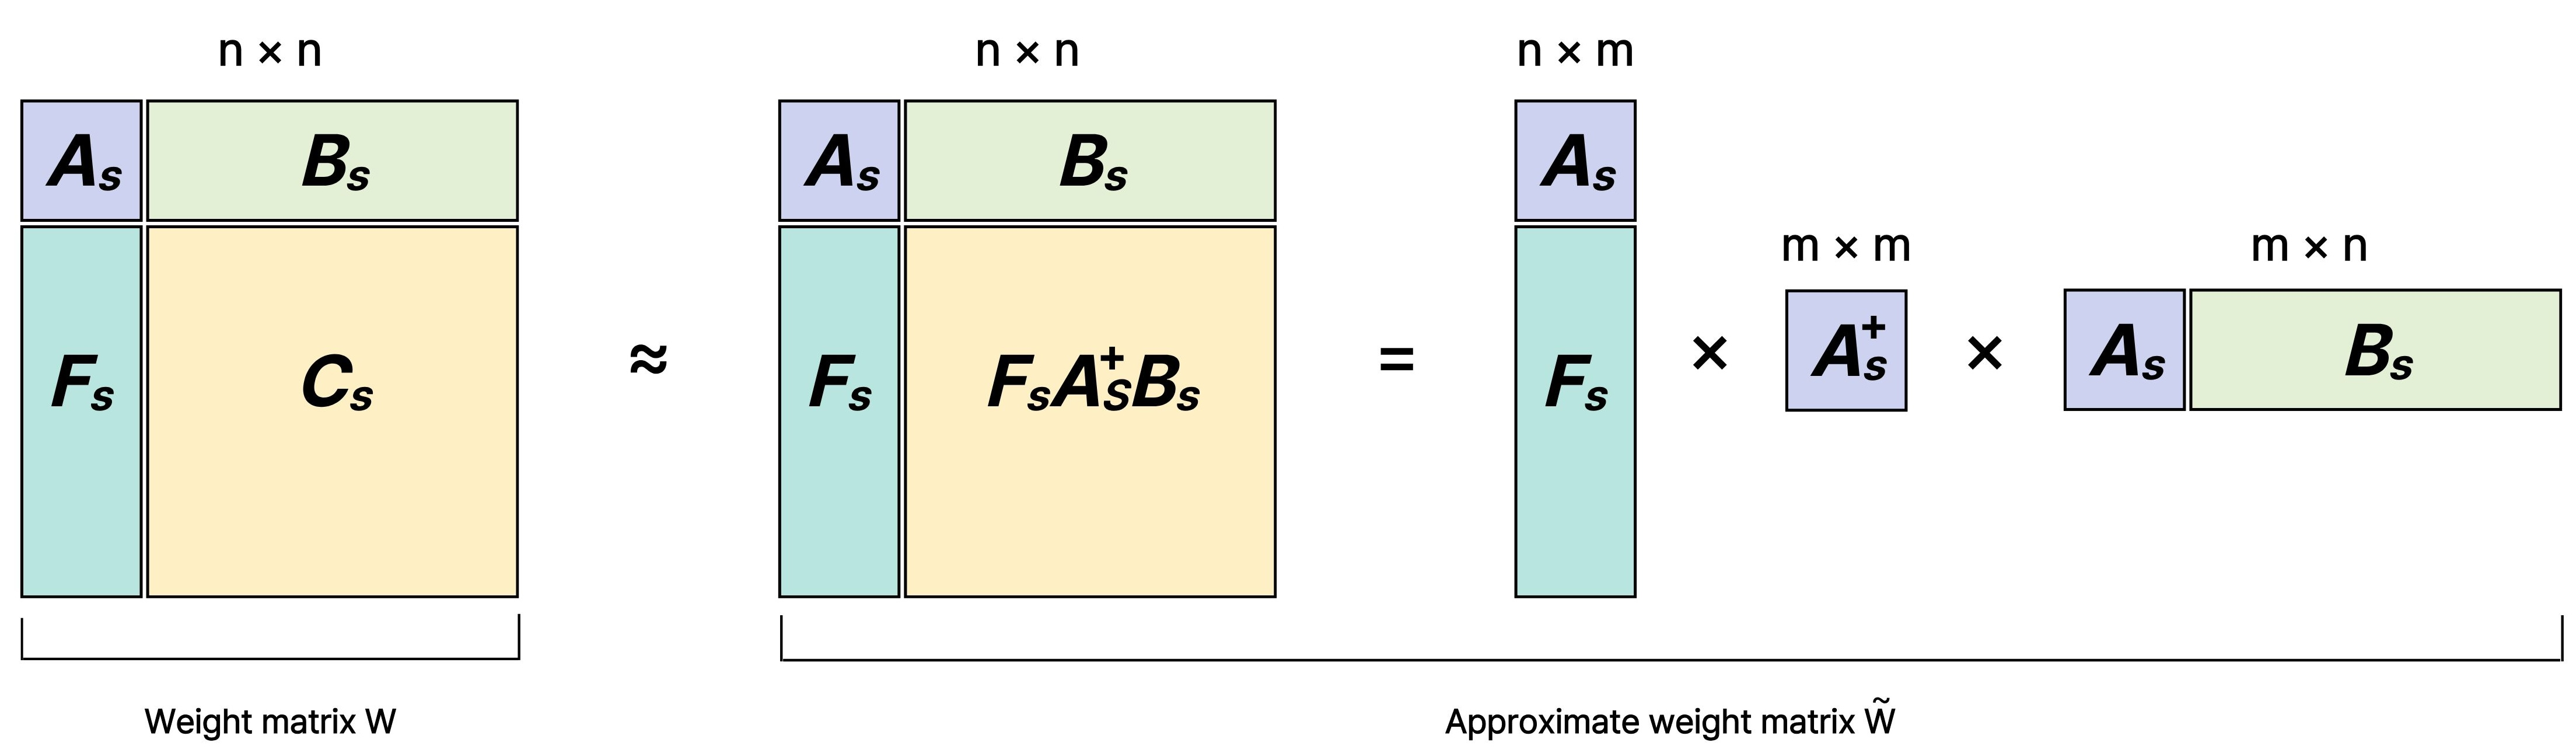
\includegraphics[width=\columnwidth]{../images/nystrom-approx.jpg}%
    }\\[6pt]
    \subfloat[Our \name{} Freivalds' check\label{fig:zkdiet}]{%
        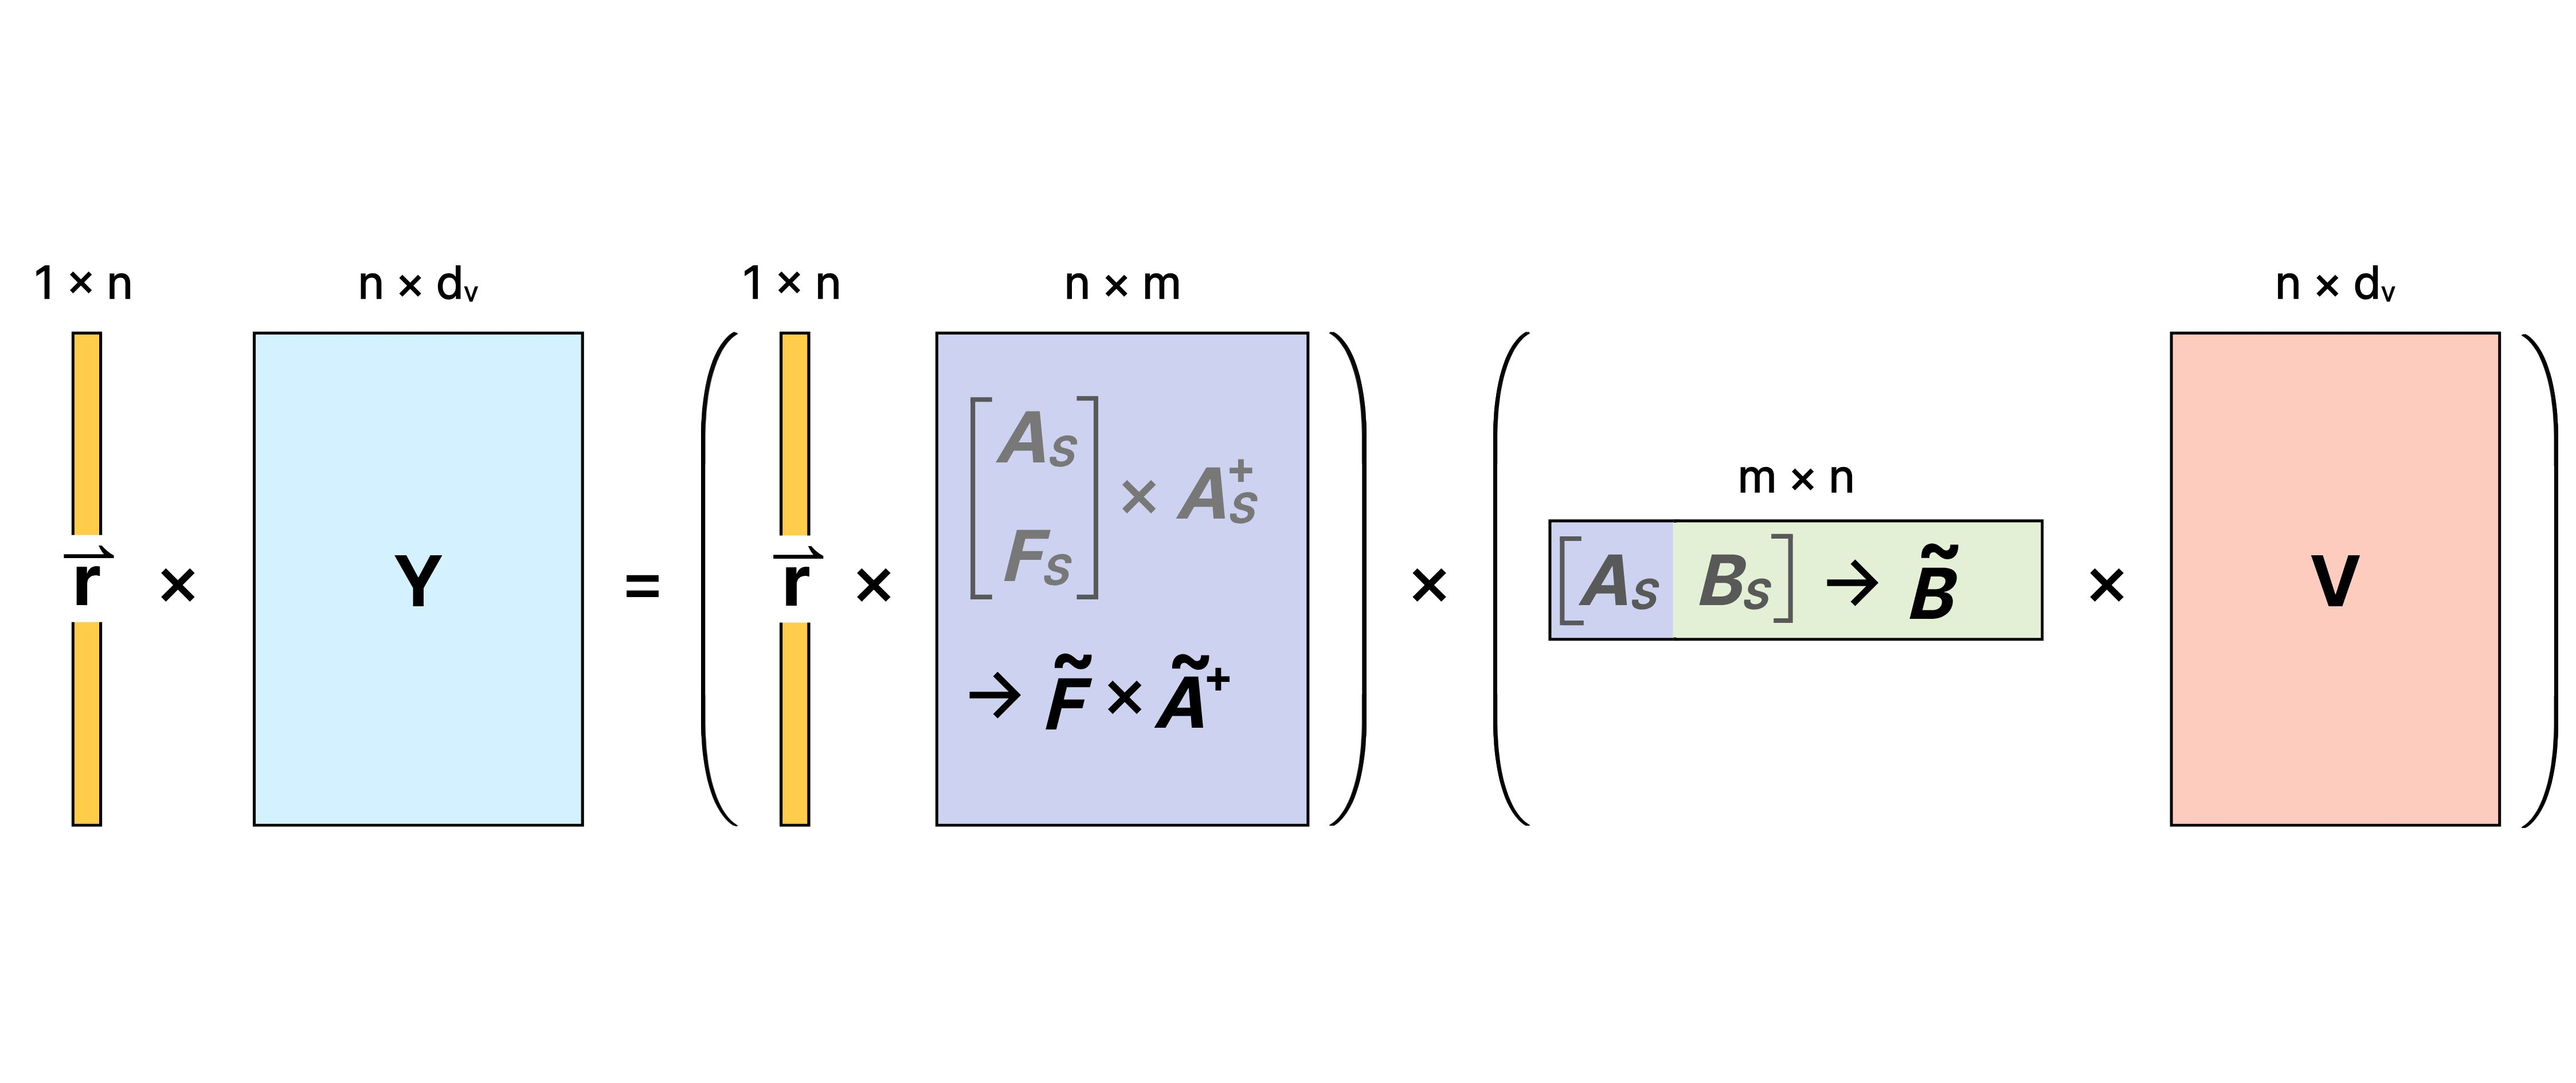
\includegraphics[width=\columnwidth]{../images/zkdiet-freivalds.jpg}%
    }
    \caption{Low-rank matrix multiplication with Freivalds' algorithm (illustrated for Nystr\"omformer). Other instances decompose the attention matrix differently (Table~\ref{tab:instances}).}
    \label{fig:chain}
\end{figure}

\paragraph{Low-rank factor chain.}
As illustrated in Figure~\ref{fig:nystrom-approx}, rather than directly handling the $n \times n$ self-attention matrix, we follow the Nystr\"omformer procedure and decompose it into a sequence of low-dimensional matrices of shapes $n \times m$, $m \times m$, and $m \times n$. We denote the three low-rank factors by
$\tilde{F} := \sfmax(\Q\widetilde{\K}^{\top}/\sqrt{d_k}) \in \mathbb{F}^{n \times m}$,
$\tilde{A} := \sfmax(\widetilde{\Q}\widetilde{\K}^{\top}/\sqrt{d_k}) \in \mathbb{F}^{m \times m}$, and
$\tilde{B} := \sfmax(\widetilde{\Q}\K^{\top}/\sqrt{d_k}) \in \mathbb{F}^{m \times n}$.
In the block decomposition of Figure~\ref{fig:nystrom-approx}, $\tilde{F}$, $\tilde{A}^{+}$, and $\tilde{B}$ take the roles of
$\bigl[\begin{smallmatrix} A_S \\ F_S \end{smallmatrix}\bigr]$,
$A_S^{+}$, and $\bigl[\, A_S \;\; B_S \,\bigr]$, respectively;
they are computed from the landmarks before the softmax rather than extracted from $S$ (cf.\ Section~\ref{subsec:lowrank}), so Figure~\ref{fig:zkdiet} is obtained from Figure~\ref{fig:nystrom-approx} by this substitution. The chain is thus $\Y = \tilde{F}\tilde{A}^{+}\tilde{B}\V$ with $G_1 = \tilde F$, $G_2 = \tilde A^{+}$, and $G_3 = \tilde B$.

\paragraph{Freivalds' checks.}
By applying Freivalds' algorithm to this low-rank representation (Figure~\ref{fig:zkdiet}), we compress the verification workload from $\mathcal{O}(n^2)$ to $\mathcal{O}(n)$, effectively reducing it to a chain of vector--matrix products of total size $2nm + m^2 + nd_v$: multiplying the random vector by $\tilde{F}$ ($nm$), then by $\tilde{A}^{+}$ ($m^2$), then by $\tilde{B}$ ($mn$), and finally by~$\V$ ($nd_v$). In the formal relation, this chain is verified in three fixed-point rescaled stages, with the two intermediate products committed (Section~\ref{moore-penrose}).

\paragraph{Non-linearities and the pseudoinverse witness.}
The softmax factors are enforced via lookup arguments. The pseudoinverse factor is instantiated by the iterative approximation $Z^{*}$ of Appendix~\ref{app:newton}: the prover computes $Z^{*}$ outside the circuit and supplies it as a witness, and our protocol verifies in-circuit that $Z^{*}$ satisfies the Moore--Penrose conditions (Section~\ref{moore-penrose}) up to quantization tolerance. Since these conditions uniquely characterize the pseudoinverse $\tilde{A}^{+}$, this check constrains $Z^{*}$ to a small neighborhood of $\tilde{A}^{+}$, without ever computing $\tilde{A}^{+}$ itself.

\paragraph{Other instances.}
Linformer replaces the three-factor chain by two factors, $\Y = P\,(F\V)$ with $P = \sfmax(\Q(E\K)^{\top}/\sqrt{d_k})$, so the pseudoinverse step is absent and only one softmax is enforced. SOFT keeps the three-factor shape, $\Y = B A^{+} B^{\top}\V$, with a Gaussian-kernel lookup in place of softmax and the same pseudoinverse check. In all three cases the Freivalds projections, the lookup enforcement, and the commitment structure below are unchanged (Table~\ref{tab:instances}).

\begin{figure*}[!ht]
    \centering
    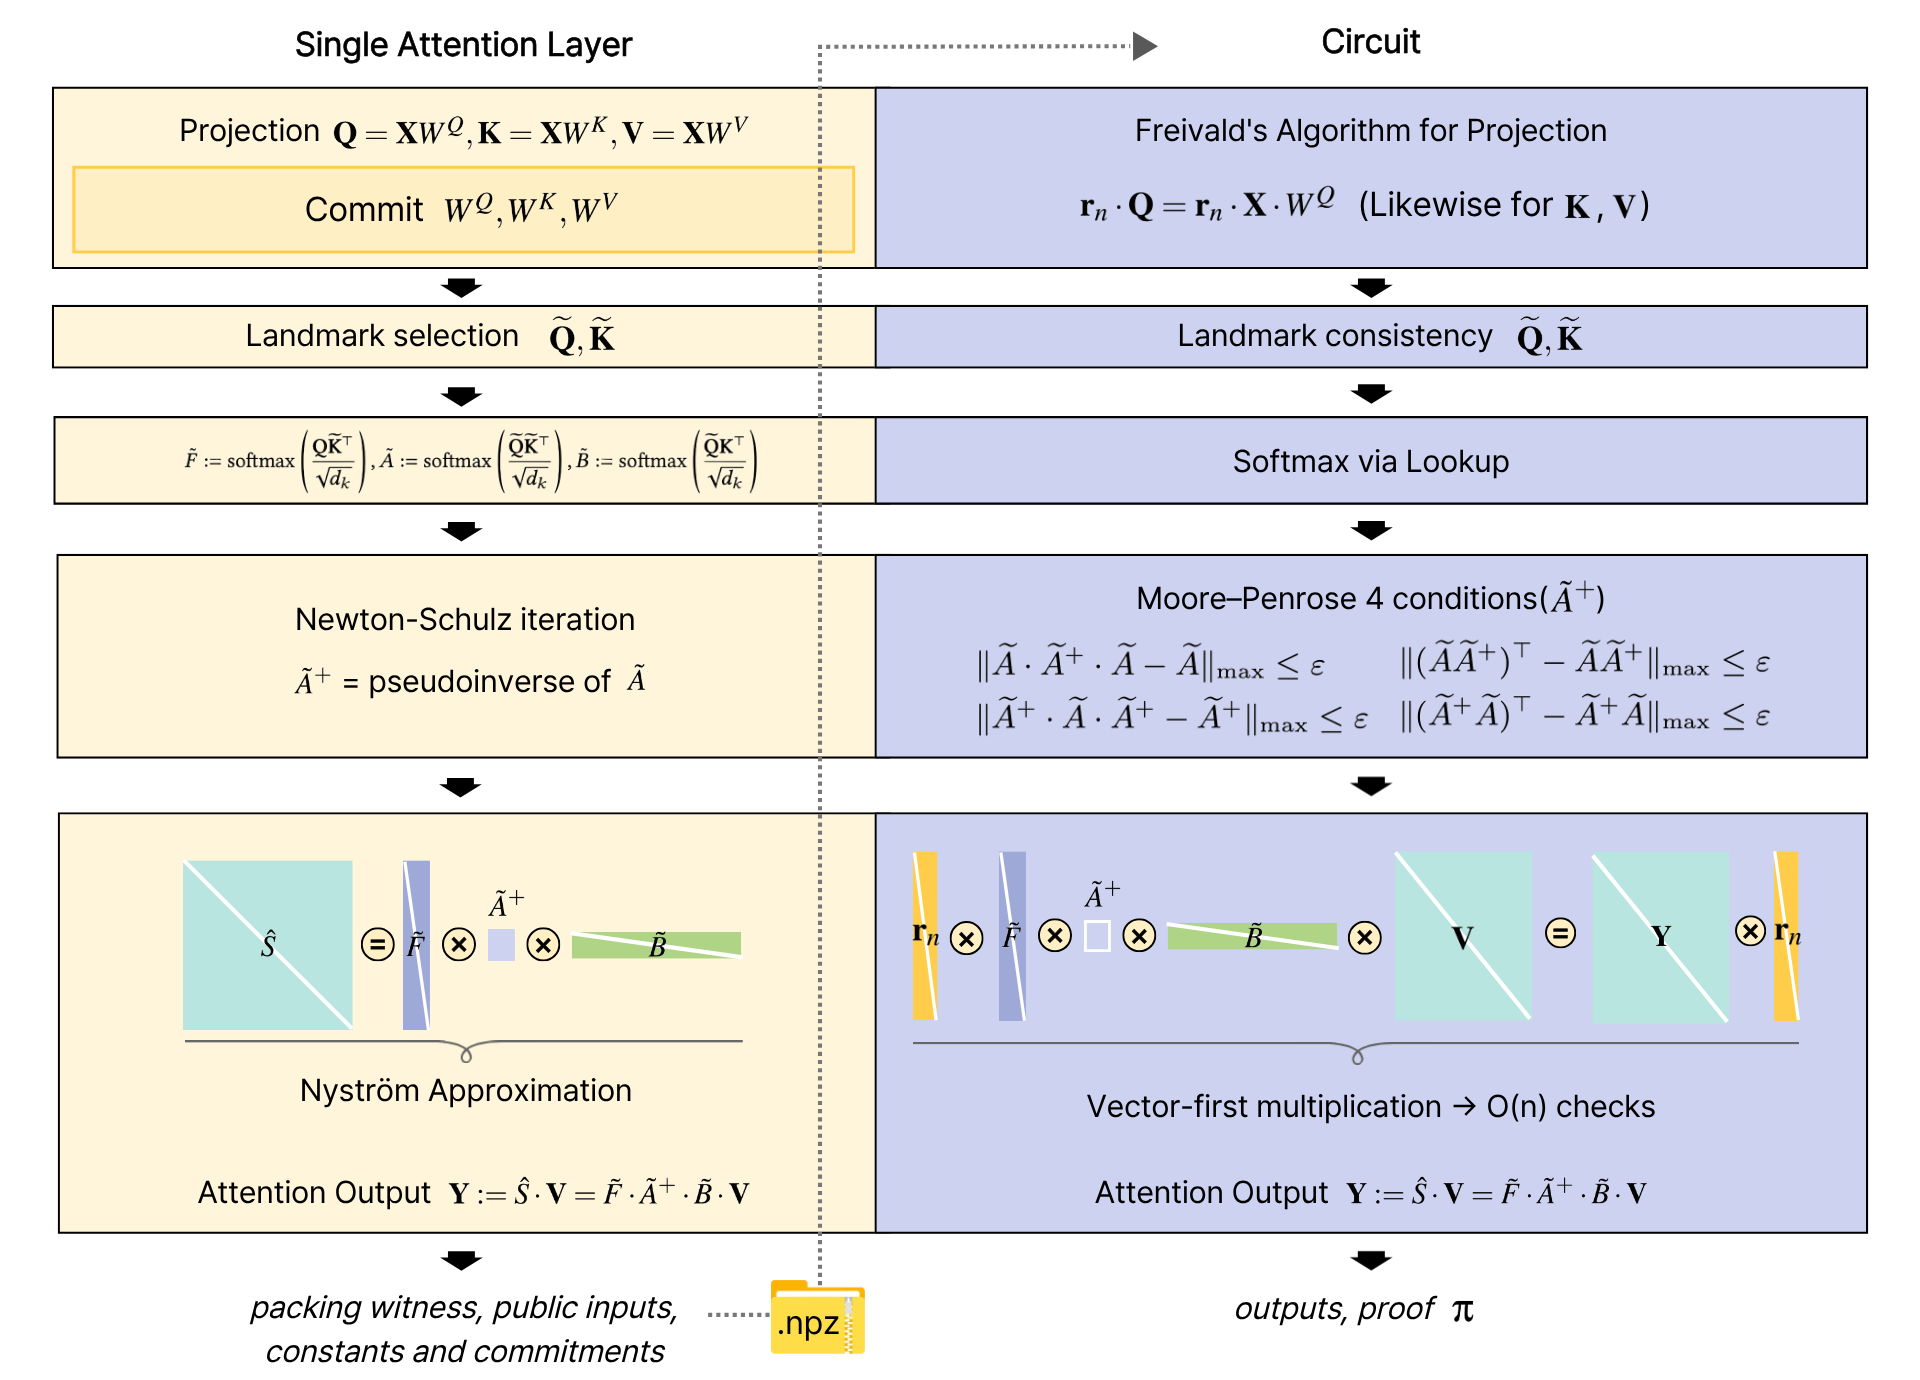
\includegraphics[width=0.9\textwidth]{../images/overview.png}
    \caption{Overview of Self-Attention and our framework}
    \label{fig:attention-overview}
\end{figure*}

\paragraph{Commit-carrying architecture.}
We embed these checks in a commit-carrying SNARK (CC-SNARK) architecture (Figure~\ref{fig:attention-overview}). Prior to serving any query, the provider publishes a global commitment $c_W \gets \Com.\commit(\ck_{\mathrm{glob}}, \W; o)$ to its weights under a circuit-independent key $\ck_{\mathrm{glob}}$.\footnote{For instances with $n$-dependent projection weights (e.g., Linformer), $c_W$ must be re-issued per sequence length; see Table~\ref{tab:instances}.} Each proof carries a circuit-dependent commitment linked to the global one via CP-linkage, so the verifier needs only constant-time checks.

For each query, the prover evaluates the attention pipeline locally, commits to the weights and intermediates under the circuit-dependent key $\ck$, sends commitments and output $\Y'$, and after receiving Freivalds challenges generates a composite proof $\pi$ encapsulating the CC-SNARK proof and two CP-linkages (Figure~\ref{fig:protocol}). In the non-interactive variant, challenges are derived via the Fiat--Shamir transformation after all commitments and $\Y'$ are fixed, preserving Freivalds' soundness.

Because zero-knowledge circuits operate over finite fields, we quantize all computations via the R1CS-friendly technique of~\cite{ZEN}. From this point onward, all matrices are over the finite field $\mathbb{F}$ after quantization.

\begin{figure*}[!ht]
\centering
\newsavebox{\protocolbox}
\savebox{\protocolbox}{%
\fbox{\procedure[head=\textbf{Protocol (Nystr\"omformer instance)}, bodylinesep=2mm]{}{
        \mathcal{P}(\ck, c_W, \X; \{ \W^Q, \W^K, \W^V, \W^O\}) \< \< \mathcal{V}(\vk, c_W, \X) \\
        (\Y', \textit{aux}, \mathsf{lk}) \gets \NystromAttention(\X, \W^Q, \W^K, \W^V, \W^O) \\
        \widetilde{\cm}_{\W^i} \gets \Com.\commit(\ck,\W^i;\tilde{o}_i) \text{ for } i \in \{Q,K,V,O\} \\
        \widetilde{\cm} \gets \Com.\commit(\ck, \mathsf{lk} ;\tilde{o}) \\
        \widetilde{\cm}_{\mathsf{aux}} \gets \Com.\commit(\ck, (\Q,\K,\V,\tilde{A}^{+},\tilde{F}\tilde{A}^{+},\tilde{B}\V,\Y) ;\tilde{o}_{\mathsf{aux}}) \\
        \<  \sendmessageright*[2cm]{\{\widetilde{\cm}_{W^i}\}_{i \in \{Q,K,V,O\}}, \widetilde{\cm}, \widetilde{\cm}_{\mathsf{aux}}, \Y'\;} \< \\
        \< \sendmessageleft*[2cm]{\rand_n, \rand_m } \< \rand_n \sample \F^n, \t \rand_m \sample \F^m  \\
        \ins := (\X, \rand_n, \rand_m, \Y') \\
        \comwit := \{ (\W^i,\tilde{o}_i)_{i \in \{Q,K,V,O\}}, (\mathsf{lk}, \tilde{o}), (\Q,\K,\V,\tilde{A}^{+},\tilde{F}\tilde{A}^{+},\tilde{B}\V,\Y,\tilde{o}_{\mathsf{aux}}) \} \\
        \uncomwit := (\widetilde{\Q}, \widetilde{\K}, \Q\widetilde{\K}^{\top}, \widetilde{\Q}\widetilde{\K}^{\top}, \widetilde{\Q}\K^{\top}) \\
        \pi \gets \Pi_\mathsf{zkdiet}.\prove( \pk, \ins; (\comwit, \uncomwit)) \\
        \<  \sendmessageright*[2cm]\pi \< \\
        \< \< \Pi_\mathsf{zkdiet}.\verify(\vk, \ins, \{\widetilde{\cm}_{W^i}\}_{i \in \{Q,K,V,O\}},\, \widetilde{\cm}, \widetilde{\cm}_{\mathsf{aux}}, c_W, \pi)
    }}%
}%
\resizebox{0.9\textwidth}{!}{\usebox{\protocolbox}}
    \caption{Protocol message flow (Nystr\"omformer instance). The structure is identical for all instances; only the attention procedure and the committed/uncommitted witness partition differ.}
    \label{fig:protocol}
\end{figure*}

\paragraph{Commit Classification Principle.}
A matrix $M$ appearing in a Freivalds-projected identity requires pre-challenge commitment ($M \in \comwit$) if and only if no element-wise in-circuit constraint uniquely determines each entry of $M$ from already-committed data. Conversely, values recoverable entry-by-entry from committed data (e.g., pre-softmax logits from lookup index and remainder-limb decomposition, or segment-averaged landmarks from committed $\Q, \K$) need no separate commitment ($M \in \uncomwit$). Table~\ref{tab:instances} lists the $\comwit$ and $\uncomwit$ partition for each instance; the soundness argument of Section~\ref{sec:security-analysis} applies this classification uniformly.

%-------------------------------------------------------------------------------
\section{\name: Efficient Proofs of Low-Rank Self-Attention via Freivalds' Algorithm}
\label{sec:protocol}
%-------------------------------------------------------------------------------

\subsection{\krev{Low-Rank Attention Pipeline}}\label{subsec:nystrom-attention}
\krev{Each instance $\mathcal{I}$ computes the attention output by (i)~projecting $\X$ to obtain $\Q,\K,\V$, (ii)~generating instance-specific low-rank factors $\{G_i\}$ from the projected tokens (Table~\ref{tab:instance-comparison}, ``Factor source'' row), (iii)~applying the instance's non-linearity (softmax or Gaussian kernel) via lookup, (iv)~supplying the pseudoinverse as a witness if required, and (v)~assembling the chain $\Y = G_1 G_2 \cdots G_j \V$ with output projection $\Y' = \Y \W^O$.}
\krev{We describe the Nystr\"{o}mformer instance in detail (Algorithm~\ref{alg:nystromAttention}); the Linformer and SOFT pipelines follow the same structure with the substitutions listed in Table~\ref{tab:instance-comparison} and Appendix~\ref{appx:instance-relations}.}


\begin{algorithm}[!t]
    \raggedright
    \scalebox{1}{
    \small
    \begin{minipage}{0.95\linewidth}
    \noindent
    \begin{tabular}{@{}l l@{}}
    \textbf{Input:} & \text{Input sequence } $\X \in \mathbb{F}^{n \times d}$, \\
    & \text{Model parameters } $\W^Q, \W^K, \W^V, \W^O \in \mathbb{F}^{d \times d}$ \\[3pt]
    \textbf{Output:} & \text{Attention output } $\Y' \in \mathbb{F}^{n \times d}$, \\
    & \text{Auxiliary intermediates } $\textit{aux}$, \\
    & \text{Non-linear operands } $\mathsf{lk} := (\tilde{F}, \tilde{A}, \tilde{B})$ \\ [2pt]
    \end{tabular}

    \underline{$\NystromAttention(\X, \W^Q, \W^K, \W^V, \W^O)$}: \\[2pt]
    $%
    \pseudocode[colspace,linenumbering]{
        \Q := \X \W^Q, \quad \K := \X \W^K, \quad \V := \X \W^V \\[2pt]
        \widetilde{\Q}, \widetilde{\K} \gets \text{SegmentAverage}(\Q, \K, m) \quad \text{(cf.\ Section~\ref{subsec:nystrom-linear})} \\[2pt]
        \tilde{F} := \sfmax\left(\frac{\Q\widetilde{\K}^\top}{\sqrt{d_k}}\right), \quad \tilde{A} := \sfmax\left( \frac{\widetilde{\Q}\widetilde{\K}^\top}{\sqrt{d_k}} \right), \quad \tilde{B} := \sfmax\left(\frac{\widetilde{\Q}\K^\top}{\sqrt{d_k}}\right) \\[2pt]
        \tilde{A}^+ \gets \computeMPInverse(\tilde{A}) \\[2pt]
        \Y := (\tilde{F} \cdot \tilde{A}^+) (\tilde{B} \cdot \V) \\[2pt]
        \Y' := \Y \cdot \W^O \\[2pt]
        \textit{aux} := (\Q, \K, \V, \widetilde{\Q}, \widetilde{\K}, \Q\widetilde{\K}^\top, \widetilde{\Q}\widetilde{\K}^\top, \widetilde{\Q}\K^\top, \tilde{A}^+, \tilde{F}\tilde{A}^{+}, \tilde{B}\V, \Y) \\[2pt]
        \mathsf{lk} := (\tilde{F}, \tilde{A}, \tilde{B}) \\[2pt]
        \pcreturn (\Y', \textit{aux}, \mathsf{lk})
    }%
    $
    \end{minipage}
    }
    \caption{\nystrom approximation of attention matrix}
    \label{alg:nystromAttention}
\end{algorithm}

\subsection{Efficient Verification via Freivalds' Algorithm}
\label{moore-penrose}
Our protocol uses Freivalds' algorithm as a core tool to efficiently verify that the low-rank self-attention computation is performed correctly. In particular, within the zk-SNARK circuit, we employ Freivalds' algorithm to ensure that the following key operations can be verified with linear cost. \\

\sss{Query/Key/Value matrix generation and output projection}
Using the verifier's random vector $\rand_n$, we check the relation $\Q = \X \W^Q$ by comparing $\rand_n^{\top} \Q$ with $\rand_n^{\top}(\X \W^Q)$.
We verify $\K$ and $\V$ in the same way. Rather than proving the full $n\times d$ matrix product directly, this Freivalds' check reduces verification to computing only the vector-matrix product $\rand_n^{\top}\X \W^Q$, thereby reducing the complexity from $\mathcal{O}(n d^2)$ to $\mathcal{O}(nd + d^2)$. The output projection $\Y'=\Y \W^O$ is verified analogously: we check $\rand_n^{\top}\Y' \stackrel{?}{=} (\rand_n^{\top}\Y)\,\W^O$. \\

\sss{\krev{Instance-specific factor products}}
\krev{Each instance requires $N_{\mathcal{I}}{-}4$ additional Freivalds checks beyond the four common projection identities (Table~\ref{tab:instance-comparison}). For example, Nystr\"{o}mformer verifies $\Q\widetilde{\K}^{\top}$, $\widetilde{\Q}\widetilde{\K}^{\top}$, $\widetilde{\Q}\K^{\top}$; Linformer verifies $E_i\K$, $F_i\V$, $\Q(E\K)^{\top}$. Each product is checked by multiplying both sides with a random vector of matching dimension:}
\[
\rand_n^{\top}\!\bigl(\Q\widetilde{\K}^{\top}\bigr)
\stackrel{?}{=}
(\rand_n^{\top}\Q)\,\widetilde{\K}^{\top}
\]
\krev{reducing verification to vector-matrix products without materializing any $n \times n$ matrix in the circuit.} \\

% TODO(MP): "four" -> "three (cond 1,3,4)" once MP enforcement confirmed
\sss{Moore--Penrose pseudoinverse}
\krev{For instances employing a pseudoinverse (Nystr\"{o}mformer, SOFT; Table~\ref{tab:instance-comparison}, ``Pseudoinverse'' row), computing $A_\mathcal{I}^{+}$ inside the circuit is inefficient.} Instead, the prover supplies $\tilde{A}^{+}$ as a witness, and the circuit verifies the four Moore--Penrose conditions \krev{(line~10 of Figure~\ref{fig:relation})} as element-wise range checks $\lVert\cdot\rVert_{\max}\leq\varepsilon$, where the tolerance $\varepsilon$ is determined by the \krev{iterative procedure (Appendix~\ref{appx:newton-schulz})}; the concrete value is specified in Section~\ref{subsec:pseudoinverse} (exact in-circuit computation is negligible: $\mathcal{O}(m^3)$ field operations for $m{=}32$). \krev{For Linformer, no pseudoinverse is required and this step is absent.}

\krev{The relations that the prover must satisfy are formalized in Figure~\ref{fig:relation} as the generalized circuit relation $\R_\mathcal{I}$, parametrized by the attention instance. The public instance is $\ins=(\X,\rand,\Y')$ and the witness $\wit=(\comwit_\mathcal{I}, \uncomwit_\mathcal{I})$. The Commit Classification Principle (Section~\ref{sec:overview}) determines the partition: $\comwit_\mathcal{I}$ includes all values requiring pre-challenge commitment (weights, lookup operands, and instance-specific auxiliary intermediates), while $\uncomwit_\mathcal{I}$ consists of values uniquely recoverable from committed data via element-wise in-circuit constraints. Table~\ref{tab:instance-comparison} lists the partition for each instance; the full per-instance relations appear in Appendix~\ref{appx:instance-relations}. Every matrix-product identity is expressed as a Freivalds projection, reducing each check to a vector inner product.}


\begin{figure}[t!]
\center
\fbox{\procedure[
    head=\textbf{Generalized Relation},
    bodylinesep=2mm,
    linenumbering,
    mode=text
]{}{
        $\R_{\mathcal{I}}(\ins, \wit): $\\[2pt]
        $\t \pcparse \ins = (\X, \rand, \Y'), \wit = (\comwit_{\mathcal{I}}, \uncomwit_{\mathcal{I}})$ \\[4pt]
        \text{\% --- Common prefix (all instances) ---} \\
        $\t \rand_n^\top \cdot \Q = \rand_n^\top \cdot \X \cdot \W^Q$ \\
        $\t \rand_n^\top \cdot \K = \rand_n^\top \cdot \X \cdot \W^K$ \\
        $\t \rand_n^\top \cdot \V = \rand_n^\top \cdot \X \cdot \W^V$ \\[4pt]
        \text{\% --- Instance-specific middle (see Table~\ref{tab:instance-comparison} and Appendix~\ref{appx:instance-relations}) ---} \\
        $\t \text{(a) Factor generation: } \{G_i\}_{i=1}^{j_{\mathcal{I}}} \text{ from } \Q, \K, \V \text{ (instance-specific)}$ \\
        $\t \text{(b) Factor product verification via Freivalds (}N_{\mathcal{I}}{-}4 \text{ identities)}$ \\
        $\t \text{(c) Non-linearity enforcement (softmax / Gaussian kernel)}$ \\
        $\t \text{(d) Witness verification (MP conditions if pseudoinverse used; }\varepsilon_{\mathcal{I}}\text{-tolerant)}$ \\
        $\t \text{(e) Chain assembly: } \rand_n^\top \cdot \Y = \rand_n^\top \cdot G_1 G_2 \cdots G_{j_{\mathcal{I}}} \cdot \V$ \\[4pt]
        \text{\% --- Common suffix ---} \\
        $\t \rand_n^\top \cdot \Y' = \rand_n^\top \cdot \Y \cdot \W^O$
}}
\caption{\krev{Generalized relation of \name, parametrized by the attention instance $\mathcal{I}$. Lines~3--5 and~12 are common to all instances; lines~7--11 are instantiated per Table~\ref{tab:instance-comparison}. Full per-instance relations appear in Appendix~\ref{appx:instance-relations}. All projected checks use fixed-point quotient-remainder decompositions with remainders range-checked to $[0, 2^{k_{\mathrm{bits}}})$.}}
\label{fig:relation}
\end{figure}

\begin{table}[t!]
\centering
\caption{\krev{Instance comparison for the three supported low-rank attention mechanisms. $N_{\mathcal{I}}$ counts all Freivalds-projected identities including Q/K/V and output projection checks as well as the pseudoinverse verification matmuls (4 per pseudoinverse, verifying the intermediate products used in the MP element-wise checks).}}
\label{tab:instance-comparison}
\resizebox{\columnwidth}{!}{%
\footnotesize
\setlength{\tabcolsep}{3pt}
\begin{tabular}{@{} l ccc @{}}
\toprule
& \textbf{\nystromformer} & \textbf{Linformer} & \textbf{SOFT} \\
\midrule
Attention output
  & $\tilde{F}\,\tilde{A}^{+}\tilde{B}\,\V$
  & $P\,F\V$
  & \krev{$B\,A^{+}B^{\top}\V$} \\[2pt]
Low-rank factors
  & \krev{3 kernel ($\tilde{F},\tilde{A},\tilde{B}$) + $\tilde{A}^{+}$}
  & 2 ($EK, FV$) + logit
  & \krev{2 kernel ($B, A$) + $A^{+}$} \\[2pt]
Factor dimensions
  & $n{\times}m,\, m{\times}m,\, m{\times}n$
  & $k{\times}d,\, k{\times}d,\, n{\times}k$
  & $n{\times}m,\, m{\times}m,\, m{\times}n$ \\[2pt]
Factor source
  & Input-derived (seg.\ avg.)
  & Learned ($E_i, F_i$)
  & \krev{Input-derived (seg.\ avg., $\Q$ only)} \\[2pt]
Non-linearity
  & softmax $\times 3$
  & softmax $\times 1$
  & \krev{Gaussian kernel $\times 2$} \\[2pt]
Pseudoinverse
  & $\tilde{A}^{+}$ (Newton--Schulz)
  & None
  & \krev{$A^{+}$ (Newton--Raphson, $T{=}20$)} \\[2pt]
MP conditions
  & \krev{3 (cond.\ 1,3,4; $\varepsilon$-tol.)}
  & 0
  & \krev{3 (cond.\ 1,3,4; $\varepsilon$-tol.)} \\[2pt]
Freivalds ($N_{\mathcal{I}}$)
  & \krev{14}
  & 8
  & \krev{12} \\[2pt]
Cross-$n$ binding
  & Yes
  & No ($E_i,F_i$ are $k{\times}n$)
  & Yes \\
\bottomrule
\end{tabular}%
}
\end{table}

\section{Security}
\label{sec:security}

\krev{In this section, we formalize the security guarantees provided by \name. We outline the system and threat models (Section~\ref{subsec:threat-model}), present our security definition (Section~\ref{subsec:sec-def}), and sketch the proof of Theorem~\ref{thm:security} (Section~\ref{sec:security-analysis}).}

\subsection{System and Threat Model}
\label{subsec:threat-model}

\krev{Our system involves two parties, a \emph{model provider} and a \emph{user}. The provider holds the trained per-layer weight matrices $\W$ of a Transformer with low-rank attention (instance $\mathcal{I}$) and exposes an inference interface: the user submits an input sequence $\X \in \mathbb{F}^{n \times d}$ and receives the corresponding output $\Y'$. The architectural parameters $\mathsf{zkdiet} = (n, d, h, L, m_{\mathcal{I}}, k_{\mathrm{bits}})$, including the low-rank dimension $m_{\mathcal{I}}$ and the quantization precision, are public and fixed by the circuit; only the weight values are private. For instances with $n$-independent weights (Nystr\"{o}mformer, SOFT), the provider publishes a single commitment $c_{W}$ under a circuit-independent key, so that responses across different sequence lengths are bound to one model. For instances with $n$-dependent projection weights (Linformer), $c_W$ must be re-issued for each sequence length (Table~\ref{tab:instance-comparison}, ``Cross-$n$ binding'' row).}

\krev{We denote the resulting functionality by $\Y' \leftarrow \mathcal{F}^{\varepsilon_\mathcal{I}}_{\mathsf{zkdiet}}(\W, \X)$, where $\mathcal{F}^{\varepsilon_\mathcal{I}}_{\mathsf{zkdiet}}$ is the quantized low-rank attention pipeline of instance $\mathcal{I}$ (Figure~\ref{fig:relation}), and $\varepsilon_\mathcal{I}$ is the residual tolerance admitted for instances employing a pseudoinverse witness ($\varepsilon_\mathcal{I}{=}0$ for Linformer).}

A zero-knowledge verifiable low-rank attention inference ($\mathsf{zkDIET}$) scheme is a tuple of algorithms $\mathsf{zkDIET} = (\mathsf{KeyGen},$ $\mathsf{Setup}, \mathsf{Commit}, \mathsf{Prove}, \mathsf{Verify})$. We separate key generation into two algorithms because the two commitment layers of our protocol serve different purposes: one binds the model across its entire lifetime, the other binds a single proof.

\begin{itemize} [leftmargin=3mm, itemsep=2pt, topsep=2pt]
  \item $\mathsf{ck}_{\mathrm{glob}} \leftarrow \mathsf{zkDIET}.\mathsf{KeyGen}(1^{\lambda}, N)$:
        given the security parameter $\lambda$ and an upper bound $N$ on the number of field elements to be committed, output a circuit-independent commitment key. This key is sampled once and is shared by every circuit configuration the provider may later deploy.

  \item $(\mathsf{ck}, \mathsf{pk}, \mathsf{vk}) \leftarrow
        \mathsf{zkDIET}.\mathsf{Setup}(1^{\lambda}, \mathcal{R}_{\mathsf{zkdiet}})$:
        given the relation induced by the architectural parameters $\mathsf{zkdiet}$, output a circuit-dependent commitment key $\mathsf{ck}$ together with a proving key and a verification key. This algorithm is run once per architecture, not per query.

  \item $c_{W} \leftarrow
        \mathsf{zkDIET}.\mathsf{Commit}(\mathsf{ck}_{\mathrm{glob}}, \W; o)$:
        commit to the weight matrices $\W = (\W^{i})_{i \in \{Q,K,V,O\}}$ under randomness $o$. The provider publishes $c_{W}$ once, before answering any query, and reuses it across all subsequent queries and across all circuit configurations that share these weights.

  \item $(\Y', \pi) \leftarrow \mathsf{zkDIET}.\mathsf{Prove} (\mathsf{pk}, \mathsf{ck}, \mathsf{ck}_{\mathrm{glob}}, \X; \W, o)$:
        evaluate the pipeline on $\X$ outside the circuit to obtain the output $\Y'$, the non-linear operands $\mathsf{lk}$ and the auxiliary intermediates $\textit{aux}$; invoke the commit-carrying backend, which returns a proof $\pi_{cc}$ together with the proof-dependent commitments $\widetilde{\mathsf{cm}}_{W}$, $\widetilde{\mathsf{cm}}_{\mathsf{lk}}$, and $\widetilde{\mathsf{cm}}_{\mathsf{aux}}$ generated under $\mathsf{ck}$; and produce a link proof $\pi_{\mathrm{link}}$ asserting that $\widetilde{\mathsf{cm}}_{W}$ and $c_{W}$ open to the
        same weights, and that $\widetilde{\mathsf{cm}}_{\mathsf{lk}}$ and the operand commitment of the lookup argument open to the same $\mathsf{lk}$. The output
        proof is $\pi := (\pi_{cc}, \widetilde{\mathsf{cm}}_{W}, \widetilde{\mathsf{cm}}_{\mathsf{lk}}, \widetilde{\mathsf{cm}}_{\mathsf{aux}}, \pi_{\mathrm{link}})$.

  \item $\{0,1\} \leftarrow \mathsf{zkDIET}.\mathsf{Verify}(\mathsf{vk}, \X, \Y', c_{W}, \pi)$:
        accept only if $\pi_{cc}$ verifies against the public instance, the link proof holds, and the lookup argument accepts.
\end{itemize}

The verifier's trust anchor is the circuit-independent $c_{W}$, not the per-proof commitments; the link proof $\pi_{\mathrm{link}}$ bridges the two, allowing responses across different circuit configurations to be traced to the same model.

\sss{Threat Model} The two parties mutually distrust each other. The provider is \emph{malicious}: it may answer with the output of a cheaper or stale model, silently swap weights between queries or between circuit configurations, or fabricate intermediate values such as the pseudoinverse witness in order to make an incorrect output verify. The user is \emph{honest but curious}: it follows the protocol but tries to learn the weights from everything it observes, namely the published commitment, the per-proof commitments, the challenge vectors, and the proof itself. Under this model we target two properties.

\begin{itemize} [leftmargin=3mm, itemsep=2pt, topsep=2pt]
    \item \emph{Inference integrity.} An accepted $\Y'$ is the result of evaluating, under the declared architecture, the very weights fixed by the published commitment $c_{W}$, and not an arbitrary value. Since $c_{W}$ is issued once and is independent of the circuit, this binds every response the provider ever gives to a single model.
    \item \emph{Model privacy in the proof.} The transcript $\bigl(c_{W}, \widetilde{\mathsf{cm}}_{W}, \widetilde{\mathsf{cm}}_{\mathsf{lk}}, \widetilde{\mathsf{cm}}_{\mathsf{aux}}, \pi_{cc}, \pi_{\mathrm{link}}\bigr)$ leaks nothing about $\W$ beyond what $\Y'$ itself reveals.
\end{itemize}

\subsection{Security Definition}
\label{subsec:sec-def}

We keep the notation of Section~\ref{subsec:threat-model} throughout.

\begin{definition}[Zero-knowledge verifiable low-rank attention inference]
\label{def:zkdiet}
$\mathsf{zkDIET}$ is secure for $\mathcal{F}^{\varepsilon_\mathcal{I}}_{\mathsf{zkdiet}}$ if it satisfies the following three properties.
\emph{Completeness}: an honest prover always convinces the verifier.
\emph{Soundness}: no PPT adversary can make the verifier accept an output $\Y^{*}\notin\mathcal{F}^{\varepsilon_\mathcal{I}}_{\mathsf{zkdiet}}(\W^{*},\X)$ for the weights $\W^{*}$ bound by its own commitment $c_{W}^{*}$, except with negligible probability.
\emph{Zero-knowledge}: the proof transcript reveals nothing about the weights $\W$ beyond what the output $\Y'$ itself reveals; formally, there exists a PPT simulator that, given only $(\X,\Y')$, produces a transcript computationally indistinguishable from the real one.
The formal probability statements and the Real/Ideal experiment are given in Appendix~\ref{appx:security-defs}.
\end{definition}

\subsection{Security Analysis}
\label{sec:security-analysis}

\begin{theorem}[informal]
\label{thm:security}
\krev{Assume
(i)~knowledge soundness and zero-knowledge of the CC-SNARK backend and CP-link proofs,
(ii)~soundness and zero-knowledge of the lookup argument,
(iii)~binding and hiding of the commitment scheme,
(iv)~the random-oracle model for Fiat--Shamir, and
(v)~[if $\mathcal{I}$ uses a pseudoinverse:] well-conditionedness of the kernel matrix ($\sigma_{\min}(A_{\mathcal{I}}) \geq \sigma_0 > 0$).
Then, for any supported instance~$\mathcal{I}$, \textsf{zkDIET} satisfies completeness, soundness, and zero-knowledge for $\mathcal{F}^{\varepsilon_\mathcal{I}}_{\mathsf{zkdiet}}$ per Definition~\ref{def:zkdiet}. Formal statements appear in Appendix~\ref{appx:security-defs}.}
\end{theorem}

\krev{\paragraph{Soundness.}
Given an accepting transcript, knowledge soundness of the CC-SNARK yields a witness satisfying the generalized relation $\R_\mathcal{I}$ (Figure~\ref{fig:relation}); commitments and the link proof $\pi_{\mathrm{link}}$ bind the weights to $c_W$, and the lookup argument guarantees correct non-linear evaluations\footnote{\label{fn:lkp-scope}The lookup operand commitment $\widetilde{\cm}$ covers the softmax (or Gaussian kernel) operands and all range-check operands: lookup indices, fixed-point quotient-remainder decomposition remainder limbs, and division remainders from landmark generation.}. Each of the $N_\mathcal{I}$ Freivalds-projected identities (Table~\ref{tab:instance-comparison}) holds over matrices that are either public, pre-challenge committed, or uniquely determined from committed data by the Commit Classification Principle (Section~\ref{sec:overview}); Freivalds' bound gives at most $1/|\F|$ per identity. Quantization is exact in-circuit: the uniqueness of Euclidean division over the range-checked remainder pins down each quotient-remainder pair, leaving the adversary no per-entry slack. A union bound gives a total soundness error of $N_\mathcal{I}/|\F| + \negl(\lambda)$.}

\krev{\paragraph{Pseudoinverse tolerance.}
% TODO(MP): "four" -> "three (cond 1,3,4)" once MP enforcement confirmed
For instances employing a pseudoinverse (Nystr\"{o}mformer, SOFT), the Moore--Penrose conditions enforce element-wise range checks
($\lVert\cdot\rVert_{\max}\leq\varepsilon_\mathcal{I}$); these are exact in-circuit constraints contributing no additional soundness error, and $\varepsilon_\mathcal{I}$ defines the acceptance set.
Perturbation bounds~\cite{stewart1990matrix} give
$\|Z^{*} - A_\mathcal{I}^{+}\| \le O(\varepsilon_\mathcal{I}\,\|A_\mathcal{I}^{+}\|)$
under assumption~(v). For Linformer, $\varepsilon_\mathcal{I}{=}0$ and the argument reduces to the Freivalds bound alone.
The detailed argument appears in Appendix~\ref{appx:proof-sketch}.}

\paragraph{Zero-knowledge.}
The simulator $\mathcal{S}_1$ generates the CRS with its trapdoor and publishes commitments to zero, which are indistinguishable from the real ones by the hiding property. Given $(\X, \Y')$, $\mathcal{S}_2$ invokes the zero-knowledge simulators of the CC-SNARK, the link proof, and the lookup argument, and programs the random oracle so that the simulated challenges are consistent with the simulated commitments. Since every remaining transcript element is either public or simulated, the transcript reveals nothing about $\W$ beyond $\Y'$.

\krev{Orthogonal threats (model extraction, quality attestation) are discussed in Appendix~\ref{appx:out-of-scope}.}

\section{Experiments}
\label{sec:experiments}

In this section, we evaluate the concrete proof generation costs of \name and compare them against a standard self-attention baseline. Because our contribution targets the architectural cost of proving attention---i.e., the circuit structure rather than the learned weights---the evaluation focuses on the cost of the circuit itself. We use modified HuggingFace BERT and Nystr\"omformer configurations (with adjusted hidden dimensions and layer counts) to enable proving across multiple model sizes. 

\subsection{Implementation}
We implement \name in two parts: a Python-based witness generation pipeline and a Rust-based zero-knowledge proving circuit. Witness data (model weights and intermediate activations) are generated with Python~3.11.14, using PyTorch~2.9.1 and HuggingFace Transformers~4.57.3; our pipeline instruments the standard \texttt{BertForMaskedLM} and \texttt{NystromformerForMaskedLM} classes with forward hooks to capture per-layer activations. The Rust circuit is built on the arkworks library over the BLS12-381 elliptic curve and uses SHA3-256 (Keccak) for the Fiat--Shamir hash~$H$ of Section~\ref{sec:protocol} and Poseidon for in-circuit hashing.

We use LegoGroth16~\cite{Legosnark} as our commit-carrying SNARK (CC-SNARK) instantiation.  Non-arithmetic operations---softmax exponentials, SigmoidGELU activation, and LayerNorm inverse square root---are evaluated using Lasso~\cite{Lasso} lookup arguments. Theorem~\ref{thm:security} requires the lookup argument to be zero-knowledge; Lasso admits standard zero-knowledge instantiations by blinding the committed operands, and our security analysis assumes such an instantiation. Our benchmarks use the non-hiding variant, whose costs are identical up to the blinding overhead.

\sss{Pseudoinverse Computation}
\label{subsec:pseudoinverse}
As described in Section~\ref{moore-penrose}, the circuit verifies the prover-supplied $\tilde{A}^{+}$ against the Moore--Penrose conditions up to a bounded residual enforced via element-wise range checks.
We empirically evaluated the maximum element-wise residual under a tiny-spec configuration ($m{=}32$ landmarks and $12$-bit quantization).
The observed maximum residuals for the verified conditions range from $1$ to $161$ relative to the full quantization range $[0, 4095]$.
To accommodate these residuals, the circuit enforces bounds of $\varepsilon \in \{4, 64, 512\}$, providing a $3\times$ to $5\times$ safety margin above the empirical maximum errors, which strictly remain below $4\%$ of the full range; the analysis of Section~\ref{sec:security-analysis} conservatively takes $\varepsilon$ to be the largest of these per-condition bounds.

\sss{Quantization}
\label{subsec:quantization}
As noted in Section~\ref{sec:overview}, we quantize all model computations following the R1CS-friendly quantization scheme of ZEN~\cite{ZEN}. All weights and activations are converted to 12-bit asymmetric fixed-point representations, and the circuit precision parameter is set to $k_{\text{bits}} = 26$, providing sufficient headroom for accumulated multiplication errors across a full layer. Different operators use different fractional precisions to maintain numerical fidelity: LayerNorm uses 8-bit fractional precision (\texttt{FRAC\_BITS}$\,= 8$); Softmax uses 16-bit fractional precision (\texttt{FRAC\_BITS}$\,= 16$), reflecting the higher dynamic range required by the exponential function; and SigmoidGELU is evaluated via lookup tables of size $2^{16} = 65{,}536$ entries.
For circuit efficiency we replace GELU with the lookup-friendly SigmoidGELU variant in all layers of both models; the definition and rationale are given in Appendix~\ref{appx:mlp-costs}.

\subsection{Experimental Configuration}
\label{subsec:configuration}

\sss{Hardware}
All experiments run on a Mac Studio with an Apple M1 Ultra (20 cores) and 128\,GB unified memory (CPU only; no GPU). Timing is CPU wall-clock via Rayon's thread pool; peak memory is the maximum RSS reported by the system \texttt{time} utility.

\sss{Baselines and Configurations}
We compare two HuggingFace~\cite{HuggingFace} architectures---\texttt{BertForMaskedLM}~\cite{BERT} ($\mathcal{O}(n^2d)$ attention) and \texttt{NystromformerForMaskedLM}~\cite{Nystromformer} ($\mathcal{O}(n)$ attention)---across five BERT-family configurations (Table~\ref{tab:model_configs}). Both share identical $(L, d, h)$ per scale, differing only in the attention kernel.
\begin{table}[t]
    \centering
    \footnotesize
    \begin{tabular}{c c c c}
    \hline
    Model & $L$ & $d$ & $h$ \\
    \hline
    Tiny   & 2  & 128 & 2 \\
    Mini   & 4  & 256 & 4 \\
    Small  & 4  & 512 & 8 \\
    Medium & 8  & 512 & 8 \\
    Base   & 12 & 768 & 12 \\
    \hline
    \end{tabular}
    \caption{Model configurations across the standard BERT family (Tiny to Base)}
    \label{tab:model_configs}
\end{table}


\subsection{Results}
\label{subsec:pipeline-costs}
All reported metrics are \emph{per single layer}: each table entry is the average of the per-layer measurements across all~$L$ layers of the model (e.g., $L{=}2$ for Tiny). Timing values (setup, commit, prove, verify) and proof size are averaged over the $L$~layers. Memory denotes the peak resident set size (RSS) observed during a single process that proves all $L$ layers sequentially; because it is a process-wide maximum, it is \emph{not} averaged but reported as a single value. We measure six sequence lengths $n \in \{128, 256, 512, 1024, 2048, 4096\}$ with a fixed landmark count $m{=}32$ for \nystrom attention. Table~\ref{tab:master} reports the full-pipeline sweep, which exhausts memory beyond $n{=}1024$; the attention-only sweep of Figure~\ref{fig:bert-vs-nystrom-freivalds} extends to $n{=}4096$. This range is chosen to expose the asymptotic advantage of Nystr\"om attention over standard self-attention: since the landmark count $m$ is held fixed while $n$ varies, the Nystr\"om approximation scales as $\mathcal{O}(n)$ in both time and memory~\cite{Nystromformer}, whereas standard self-attention scales as $\mathcal{O}(n^2)$. For each circuit instance, we report constraint count, setup time, prove time, verify time, peak memory, and two commitment costs: the Groth16 committing time (G16) for committing to the committed witness slice---the weights and the intermediate matrices ($\Q$, $\K$, $\V$, $\tilde{A}^{+}$, $\tilde{F}\tilde{A}^{+}$, $\tilde{B}\V$, $\Y$), and the Lasso committing time for committing to the lookup operands. The global commitment to the model weights is a one-time cost independent of the number of layers and is therefore excluded from the per-layer metrics; in our measurements it takes approximately $965$\,ms. Runs that exceed available memory are reported as out-of-memory (OOM); these patterns are themselves informative results, as they indicate the practical scalability boundary of each circuit variant. We evaluate \name by applying its two constituent techniques---low-rank (\nystrom) attention and Freivalds-based matrix-multiplication verification---one at a time, first isolating each technique's individual contribution and then combining both to measure the advantage of the full scheme.
In our benchmarks, we pass only cryptographic hashes of the input sequence $\X$ and the attention output $\Y'$ as the public instance, while supplying $\X$ and $\Y'$ themselves as witnesses. This approach avoids the prohibitive setup cost incurred by large public-input vectors. Note that this is a deployment-time configuration; the protocol definition in Figure~\ref{fig:protocol} presents $\X$ and $\Y'$ directly as public instances for clarity. Soundness is preserved under the collision resistance of the hash: the Fiat--Shamir transcript binds the hashed instance, so the fixed-before-challenge argument of Section~\ref{sec:security-analysis} carries over.

\begin{table}[!ht]
\centering
\caption{Full $2{\times}2$ factorial design---attention kernel (BERT / \nystrom) $\times$ matrix-multiplication verification (Naive / Freivalds)---on the Tiny configuration ($L{=}2$, $d{=}128$, $h{=}2$). All metrics are per single layer (averaged over $L$ layers). OOM entries (---) indicate that setup exhausted 128\,GB; for these runs the Peak RAM column reports the observed process-wide maximum before termination. The G16 column reflects the extended committed slice (weights $+$ $\Q, \K, \V, \tilde{A}^{+}, \tilde{F}\tilde{A}^{+}, \tilde{B}\V, \Y$).}
\label{tab:master}
\resizebox{\columnwidth}{!}{%
\small
\setlength{\tabcolsep}{3pt}
\begin{tabular}{@{} cl rrrrrrrrr @{}}
\toprule
 & & & & \multicolumn{2}{c}{Commit (ms)} & & & & \\
\cmidrule(lr){5-6}
$n$ & Configuration & Constr.\ (M) & Setup (s) & G16 & Lasso & Prove (s) & Verify (ms) & Proof (KB) & RAM (GB) \\
\midrule
\multirow{4}{*}{128}
  & BERT-Naive     & 15.06 & 361.85 & 162.0 & 159.0 & 81.86  & 322.5 & 603.8      & 73.04 \\
  & BERT-Freivalds & 4.97  & 164.49 & 190.0 & 164.5 & 33.41  & 319.0 & 603.8      & 29.75 \\
  & Nys-Naive      & 13.47 & 344.38 & 150.0 & 268.5 & 81.41  & 570.0 & 1{,}259.9  & 68.16 \\
  & Nys-Freivalds  & 4.86  & 160.46 & 185.0 & 258.5 & 35.94  & 604.0 & 1{,}259.9  & 29.53 \\
\midrule
\multirow{4}{*}{256}
  & BERT-Naive     & 39.22 & 912.39 & 624.5 & 266.0 & 345.44 & 418.5 & 726.8      & 112.13 \\
  & BERT-Freivalds & 10.72 & 405.87 & 487.5 & 262.5 & 85.93  & 396.5 & 726.8      & 66.97 \\
  & Nys-Naive      & 26.49 & 697.46 & 275.5 & 312.0 & 187.33 & 664.5 & 1{,}346.7  & 112.18 \\
  & Nys-Freivalds  & 9.55  & 318.19 & 307.5 & 311.5 & 72.02  & 656.5 & 1{,}346.7  & 56.25 \\
\midrule
\multirow{4}{*}{512}
  & BERT-Naive     & ---   & ---    & ---       & ---   & ---    & ---   & ---        & ${>}113$ (OOM) \\
  & BERT-Freivalds & 24.79 & 920.58 & 1{,}671.5 & 622.0 & 220.52 & 624.5 & 948.3     & 112.31 \\
  & Nys-Naive      & ---   & ---    & ---       & ---   & ---    & ---   & ---        & ${>}113$ (OOM) \\
  & Nys-Freivalds  & 18.93 & 640.69 & 557.5 & 466.0 & 152.70 & 789.0 & 1{,}475.2  & 109.10 \\
\midrule
\multirow{4}{*}{1024}
  & BERT-Naive     & ---   & ---    & ---   & ---   & ---    & ---   & ---        & ${>}113$ (OOM) \\
  & BERT-Freivalds & ---   & ---    & ---   & ---   & ---    & ---   & ---        & ${>}113$ (OOM) \\
  & Nys-Naive      & ---   & ---    & ---   & ---   & ---    & ---   & ---        & ${>}113$ (OOM) \\
  & Nys-Freivalds  & 37.69 & 1{,}410.18 & 1{,}483.5 & 607.5 & 642.64 & 886.0 & 1{,}625.0  & 112.51 \\
\bottomrule
\end{tabular}%
}
\end{table}

\subsubsection{Low-Rank Attention is Essential for Asymptotic Scaling}
\label{subsec:lowrank-essential}
Fixing the verification method at naive and comparing the BERT-Naive vs.\ Nys-Naive rows of Table~\ref{tab:master} (Tiny, $L{=}2$, $d{=}128$) isolates the attention kernel's effect. At $n{=}128$ the constraint gap is modest ($15.06$M vs.\ $13.47$M, $1.1{\times}$), but by $n{=}256$ it widens to $39.22$M vs.\ $26.49$M ($1.5{\times}$) with prove time diverging from $345.44$\,s to $187.33$\,s ($1.8{\times}$). Both exhaust 128\,GB at $n{\geq}512$. The metrics on which Nys-Naive is worse than BERT-Naive---verify time, Lasso commit time, and proof size---reflect the overhead of the four Moore--Penrose checks % TODO(MP): "four" -> "three" and the three separate softmax factors; the additional proof elements, in particular, are independent of~$n$.

\subsubsection{Freivalds Removes the Constant Factor}
\label{subsec:freivalds-benefit}
Holding the kernel at \nystrom and comparing Nys-Naive vs.\ Nys-Freivalds isolates Freivalds' contribution. Across all sequence lengths, Freivalds reduces per-layer constraints by ${\sim}2.8{\times}$ (e.g., $26.49$M$\to$$9.55$M at $n{=}256$), setup time by $2.2{\times}$, and prove time by $2.6{\times}$. This ratio is stable, confirming a uniform constant-factor improvement. Freivalds extends the feasibility boundary from $n{=}256$ to $n{=}1024$ (Table~\ref{tab:master}).

\subsubsection{Freivalds Alone Cannot Substitute for Low-Rank Attention}
\label{subsec:freivalds-not-enough}
Freivalds yields comparable $3$--$3.7{\times}$ constraint reductions on BERT (Table~\ref{tab:master}), confirming it is a generic optimization. Yet BERT-Freivalds still exhausts 128\,GB at $n{\geq}1024$ because $\mathcal{O}(n^2)$ complexity remains intact, whereas Nys-Freivalds reaches $n{=}1024$. The two optimizations are therefore complementary.

\subsubsection{Combined Effect}
\label{subsec:combined-effect}
Comparing BERT-Naive with Nys-Freivalds in Table~\ref{tab:master} quantifies the joint benefit. At $n{=}256$ the combined reduction reaches $4.1{\times}$ in constraints, $2.9{\times}$ in setup, and $4.8{\times}$ in prove time, with peak memory dropping from $112.13$\,GB to $56.25$\,GB. BERT-Naive is infeasible at $n{\geq}512$, while Nys-Freivalds extends to $n{=}1024$. Full MLP\,+\,LayerNorm cost breakdowns are deferred to Appendix~\ref{appx:mlp-costs}.



\subsubsection{Multi-Spec Scaling}
\label{subsec:multi-spec}

Figure~\ref{fig:bert-vs-nystrom-freivalds} isolates the cost of proving the attention equation itself---excluding global commitment generation, weight commitment via CC-SNARK, the CP-link proof between the global and weight commitments, and Freivalds-verified $\Q$/$\K$/$\V$ projection products---and compares BERT standard attention against \nystrom attention across the full BERT model family.

The plot reports per-layer prove time (seconds) against sequence length~$n$ (linear axis) with prove time on a logarithmic axis. Each line terminates at the largest~$n$ feasible within our 128\,GB memory budget. Red lines correspond to BERT and blue lines to \nystrom. Within each color family, lighter shades represent smaller configurations and darker shades represent larger ones. Legend abbreviations: Bt/Ny $=$ BERT/\nystrom.

\begin{figure}[!ht]
\centering
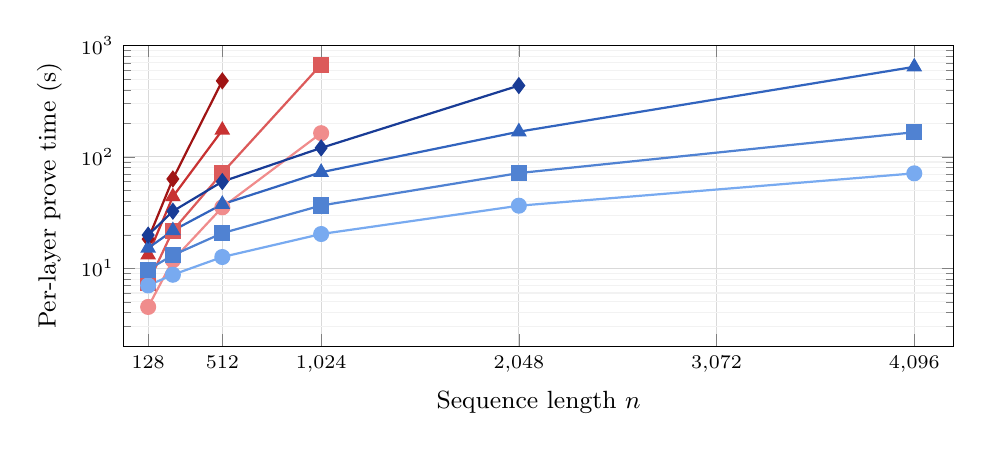
\begin{tikzpicture}
\begin{axis}[
    width=\columnwidth,
    height=5.4cm,
    ymode=log,
    log basis y=10,
    xlabel={Sequence length $n$},
    ylabel={Per-layer prove time (s)},
    xtick={128, 512, 1024, 2048, 3072, 4096},
    xmin=0, xmax=4300,
    ymin=2, ymax=1000,
    legend to name=leg:fig6,
    legend columns=4,
    legend cell align=left,
    legend style={font=\tiny, draw=none, column sep=3pt},
    label style={font=\small},
    tick label style={font=\scriptsize},
    grid=both,
    minor grid style={gray!10},
    major grid style={gray!30},
    mark size=2.5pt,
]
% === BERT attention-only (red gradient) ===
\addplot[redspec1, mark=*, thick] coordinates {
    (128,4.50) (256,11.82) (512,35.30) (1024,163.36)
};
\addlegendentry{Tiny.Bt.}
\addplot[redspec2, mark=square*, thick] coordinates {
    (128,7.38) (256,21.84) (512,71.94) (1024,674.89)
};
\addlegendentry{Mini.Bt.}
\addplot[redspec3, mark=triangle*, thick] coordinates {
    (128,13.22) (256,44.01) (512,174.09)
};
\addlegendentry{Small.Bt.}
\addplot[redspec4, mark=diamond*, thick] coordinates {
    (128,18.30) (256,63.40) (512,481.59)
};
\addlegendentry{Base.Bt.}
% === Nystrom attention-only (blue gradient) ===
\addplot[bluespec1, mark=*, thick] coordinates {
    (128,7.02) (256,8.76) (512,12.63) (1024,20.32) (2048,36.48) (4096,71.22)
};
\addlegendentry{Tiny.Ny.}
\addplot[bluespec2, mark=square*, thick] coordinates {
    (128,9.74) (256,13.12) (512,20.69) (1024,36.64) (2048,71.62) (4096,166.70)
};
\addlegendentry{Mini.Ny.}
\addplot[bluespec3, mark=triangle*, thick] coordinates {
    (128,15.21) (256,21.81) (512,37.62) (1024,72.86) (2048,168.51) (4096,643.94)
};
\addlegendentry{Small.Ny.}
\addplot[bluespec4, mark=diamond*, thick] coordinates {
    (128,19.88) (256,32.56) (512,60.03) (1024,120.50) (2048,437.00)
};
\addlegendentry{Base.Ny.}
\end{axis}
\end{tikzpicture}\\[0pt]
\ref{leg:fig6}
\caption{Per-layer prove time for the attention equation only: BERT (red) vs.\ \nystrom (blue), semi-log scale (linear $n$, logarithmic time).}
\label{fig:bert-vs-nystrom-freivalds}
\end{figure}

BERT's curves (red) rise steeply ($\mathcal{O}(n^2)$), while \nystrom (blue) grows near-linearly ($\mathcal{O}(n)$). This gap translates directly into memory exhaustion: at Base ($d{=}768$), BERT caps at $n{=}512$ while \nystrom reaches $n{=}2048$, a $4{\times}$ extension. Medium is omitted because it shares the same hidden dimension as Small ($d{=}512$), so its per-layer circuit cost is identical; only the number of layers~$L$ differs, confirming depth-invariance.

\sss{Quantization Fidelity}
\label{subsec:quantization-fidelity}
Table~\ref{tab:quantization} evaluates 26-bit fixed-point quantization ($k_\text{bits}{=}26$) on pretrained uw-madison/nystromformer-512 at $n{=}128$ over 10 batches under full cascade evaluation (errors accumulated through all 12 layers; $m{=}64$ landmarks, the model default\footnote{The circuit benchmarks in Table~\ref{tab:master} use $m{=}32$. Fidelity evaluation requires trained weights, so we adopt $m{=}64$, the default of the only publicly available pretrained checkpoint; the circuit benchmarks measure weight-independent circuit costs and therefore fix $m{=}32$.}). Top-1 agreement is $98.8$\% ($90$\% at the \texttt{[MASK]} position), top-5 is $100$\%, cosine similarity $0.9975$, confirming that 26-bit precision suffices for faithful ZK-SNARK proving.

\begin{table}[H]
\centering
\caption{Quantization fidelity of 26-bit fixed-point arithmetic on a pretrained Nystr\"omformer ($d{=}768$, 12 layers, 12 heads, $m{=}64$ landmarks) at $n{=}128$.}
\label{tab:quantization}
\footnotesize
\setlength{\tabcolsep}{4pt}
\begin{tabular}{@{} ccc cc @{}}
\toprule
\multicolumn{2}{c}{Top-1 Agree.\ (\%)} & Top-5 & Cosine & RMSE \\
\cmidrule(lr){1-2}
All pos. & Mask pos. & All (\%) & Sim. & (logit) \\
\midrule
98.8 & 90.0 & 100.0 & 0.9975 & 0.378 \\
\bottomrule
\end{tabular}
\end{table}


\subsection{Conclusion and Future Work}
\label{subsec:discussion}
Combining \nystrom low-rank attention with Freivalds verification yields multiplicative constraint savings and longer provable sequences; setup memory is the dominant bottleneck (cf.\ the OOM boundaries of Table~\ref{tab:master}). Once attention is optimized, MLP becomes the next memory frontier ($d{\geq}512$ exceeds 128\,GB; Appendix~\ref{appx:mlp-costs}).

\sss{Limitations}
\emph{(i)} CPU-only (Apple M1 Ultra); GPU proving would shift costs.
\emph{(ii)} Groth16 trusted setup is memory-bound; transparent SNARKs trade this for larger proofs.
\emph{(iii)} MLP sub-circuit remains memory-bound from $d{\geq}256$ at longer sequences.

\begin{credits}
\subsubsection{\discintname}
The authors have no competing interests to declare that are relevant to the content of this article.
\end{credits}

\bibliographystyle{splncs04}
\bibliography{references}

\appendix

\section{Newton--Schulz Iteration}
\label{appx:newton-schulz}

The prover computes the iterative approximation~$Z^{*}$ of the pseudoinverse~$\tilde{A}^{+}$ using the Newton--Schulz iteration detailed in Algorithm~\ref{alg:inverse}. The circuit does not execute this iteration; instead, % TODO(MP): "four" -> "three (cond 1,3,4)" once MP enforcement confirmed
it verifies the result via the four Moore--Penrose conditions (Section~\ref{moore-penrose}), making the iteration an off-circuit reference procedure.

\begin{algorithm}[H]
\raggedright
\scalebox{1}{
\small
\begin{minipage}{0.95\linewidth}
\textbf{Input: } $\text{selected landmark matrix } \tilde{A} \in \mathbb{F}^{m \times m}$\\
\textbf{Output: } $\text{approximate pseudoinverse }\tilde{A}^+ \in \mathbb{F}^{m \times m}$\\[2pt]
\underline{$\computeMPInverse(\tilde{A})$}: \\[2pt]
\pseudocode[colspace,linenumbering]{
  Z_0 \gets \tilde{A}^\top / \left(\|\tilde{A}\|_1 \cdot \|\tilde{A}\|_\infty\right) \\
  \text{Set } T \text{ (e.g., } T=6 \text{ iterations)} \\
  \pcfor t \in \{0,\dots,T-1\} \pcdo \\
    \t Z_{t+1} \gets \frac{1}{4} Z_t \Big( 13I - \tilde{A}Z_t\big(15I - \tilde{A}Z_t(7I - \tilde{A}Z_t)\big) \Big) \\
  \pcendfor \\
  \tilde{A}^+ \gets Z_T \\
  \pcreturn \tilde{A}^+
}
\end{minipage}
}
\caption{Compute Moore--Penrose inverse}
\label{alg:inverse}
\end{algorithm}

\section{MLP + LayerNorm Circuit Costs}
\label{appx:mlp-costs}

A complete transformer layer consists of two sub-circuits: attention and the MLP\,+\,LayerNorm block. While the main text focuses on the attention sub-circuit---the target of our \name optimizations---we additionally measured the cost of proving the MLP\,+\,LayerNorm sub-circuit, whose constraint count is the same for BERT and \nystromformer because the MLP and LayerNorm dimensions depend only on $n$ and $d$, not on the attention mechanism.

\sss{Activation Function Replacement}
One modification required by the end-to-end measurements reported in this appendix concerns the GELU activation used in the MLP block. Both BERT and \nystromformer use GELU~\cite{GELU} as their default activation, typically implemented via the approximation $\text{GELU}(x) \approx 0.5\,x\bigl(1 + \tanh\bigl[\sqrt{2/\pi}\,(x + 0.044715\,x^3)\bigr]\bigr)$.
We replace GELU in both models with SigmoidGELU, defined as
\[
    \text{SigmoidGELU}(x) = x \cdot \sigma(1.702\,x),
\]
where $\sigma(\cdot)$ denotes the logistic sigmoid. This alternative, originally noted by Hendrycks and Gimpel~\cite{GELU} as a close approximation to GELU, is substantially more circuit-friendly because the sigmoid function can be evaluated via a single lookup table, whereas the $\tanh$-based form requires a more involved computational procedure. The replacement is applied to all layers in both models.

Table~\ref{tab:mlp-costs} reports per-layer average MLP\,+\,LayerNorm costs for the Tiny configuration ($L{=}2$); all timing and memory figures are the mean of the BERT and \nystrom runs.
For larger hidden dimensions the MLP block exhausted the memory budget---at $d{\geq}512$ setup ran out of memory at all measured sequence lengths, and at $d{\geq}256$ at longer sequences---so we report the Tiny configuration only.
These measurements show that the MLP\,+\,LayerNorm sub-circuit and the attention sub-circuit contribute comparable costs at $n{=}1024$: per-layer MLP\,+\,LayerNorm proving takes $517.21$\,s versus $642.64$\,s for Nys-Freivalds attention. The MLP\,+\,LayerNorm block consumes $112.70$\,GB peak RAM at $n{=}1024$, making it a co-bottleneck alongside attention for memory-constrained environments.

For reference, proving a complete Tiny transformer layer (attention + MLP + LayerNorm) at $n{=}1024$ requires approximately $2{,}290.28$\,s of per-layer setup and $1{,}159.85$\,s of per-layer proving (${\sim}58$\,min total per layer). We report these measurements primarily as a baseline for future work on scalable ZK proving of the full transformer layer.

\begin{table}[H]
\centering
\caption{\textbf{MLP\,+\,LayerNorm} costs for the Tiny configuration ($L{=}2$, $d{=}128$).}
\label{tab:mlp-costs}
\resizebox{\columnwidth}{!}{%
\small
\setlength{\tabcolsep}{4pt}
\begin{tabular}{@{} l rrrrrrrr @{}}
\toprule
& & & \multicolumn{2}{c}{Commit (ms)} & & & & \\
\cmidrule(lr){4-5}
$n$ & Constr.\ (M) & Setup (s) & G16 & Lasso & Prove (s) & Verify (ms) & Proof (KB) & RAM (GB) \\
\midrule
128  & 0.98  & 95.10  & 116.0 & 150.3 & 28.69  & 287.5 & 520.7      & 26.46 \\
256  & 1.96  & 189.64 & 217.8 & 172.3 & 58.84  & 309.5 & 572.8      & 53.31 \\
512  & 3.92  & 385.39 & 438.0 & 295.3 & 138.99 & 409.5 & 654.6      & 101.55 \\
1024 & 7.84  & 880.10 & 1{,}128.3 & 426.5 & 517.21 & 477.3 & 746.1     & 112.70 \\
\bottomrule
\end{tabular}%
}
\end{table}

\section{Formal Security Definitions}
\label{appx:security-defs}

We state the formal probability conditions for the three security properties of Definition~\ref{def:zkdiet}. Notation follows Section~\ref{subsec:threat-model}.

\smallskip
\noindent\emph{Completeness.} For every $\W = (\W^{i})_{i \in \{Q,K,V,O\}}$ with each $\W^{i} \in \mathbb{F}^{d \times d}$ and every $\X \in \mathbb{F}^{n \times d}$, for $\mathsf{ck}_{\mathrm{glob}} \leftarrow \mathsf{KeyGen}(1^{\lambda}, N)$, $(\mathsf{ck}, \mathsf{pk}, \mathsf{vk}) \leftarrow \mathsf{Setup}(1^{\lambda}, \mathcal{R}_{\mathsf{zkdiet}})$, $c_{W} \leftarrow \mathsf{Commit}(\mathsf{ck}_{\mathrm{glob}}, \W; o)$ and $(\Y', \pi) \leftarrow \mathsf{Prove}(\mathsf{pk}, \mathsf{ck}, \mathsf{ck}_{\mathrm{glob}}, \X; \W, o)$,
\[
    \Pr\bigl[\mathsf{Verify}(\mathsf{vk}, \X, \Y', c_{W}, \pi) = 1\bigr] = 1 .
\]

\noindent\emph{Soundness.} For any PPT adversary $\mathcal{A}$, there exists a PPT extractor $\mathcal{E}$ such that
\[
  \Pr \left[
  \begin{array}{c}
    \mathsf{Verify}(\mathsf{vk}, \X, \Y^{*}, c_{W}^{*}, \pi^{*}) = 1 \\[2pt]
    \land\ \ c_{W}^{*} = \mathsf{Commit}(\mathsf{ck}_{\mathrm{glob}}, \W^{*}; o^{*}) \\[2pt]
    \land\ \ \Y^{*} \notin \mathcal{F}^{\varepsilon_\mathcal{I}}_{\mathsf{zkdiet}}(\W^{*}, \X)
  \end{array}
  \;\middle|\;
  \begin{array}{l}
    \mathsf{ck}_{\mathrm{glob}} \leftarrow \mathsf{KeyGen}(1^{\lambda}, N) \\[2pt]
    (\mathsf{ck}, \mathsf{pk}, \mathsf{vk}) \leftarrow \mathsf{Setup}(1^{\lambda}, \mathcal{R}_{\mathsf{zkdiet}}) \\[2pt]
    (c_{W}^{*}, \X, \Y^{*}, \pi^{*}) \leftarrow \mathcal{A}(\mathsf{ck}_{\mathrm{glob}}, \mathsf{ck}, \mathsf{pk}, \mathsf{vk}) \\[2pt]
    (\W^{*}, o^{*}) \leftarrow \mathcal{E}^{\mathcal{A}}(\mathsf{trans}_{\mathcal{A}})
  \end{array}
  \right] \le \mathsf{negl}(\lambda).
\]

\noindent\emph{Zero-knowledge.}
Write $\mathsf{Eval}(\W, \X)$ for the deterministic off-circuit evaluation of Algorithm~\ref{alg:nystromAttention}. There exists a PPT simulator $\mathcal{S} = (\mathcal{S}_{1}, \mathcal{S}_{2})$ such that for every $\W$ and every PPT adversary $\mathcal{A} = (\mathcal{A}_{1}, \mathcal{A}_{2})$, the two experiments below are computationally indistinguishable (barred symbols denote simulator-produced values):
\[
\begin{array}{@{}l@{\qquad}l@{}}
\underline{\mathsf{Real}_{\mathcal{A}, W}(\lambda)} &
\underline{\mathsf{Ideal}_{\mathcal{A}, \mathcal{S}, W}(\lambda)} \\[4pt]
\mathsf{ck}_{\mathrm{glob}} \leftarrow \mathsf{KeyGen}(1^{\lambda}, N) &
(\overline{\mathsf{ck}}_{\mathrm{glob}}, \overline{\mathsf{ck}},
 \overline{\mathsf{pk}}, \overline{\mathsf{vk}}, \overline{c}_{W},
 \mathsf{td}) \leftarrow
 \mathcal{S}_{1}(1^{\lambda}, N, \mathcal{R}_{\mathsf{zkdiet}}) \\
(\mathsf{ck}, \mathsf{pk}, \mathsf{vk}) \leftarrow
 \mathsf{Setup}(1^{\lambda}, \mathcal{R}_{\mathsf{zkdiet}}) & \\
o \xleftarrow{\$} \mathcal{O};\ \
 c_{W} \leftarrow \mathsf{Commit}(\mathsf{ck}_{\mathrm{glob}}, \W; o) & \\
(\X, st) \leftarrow \mathcal{A}_{1}(\mathsf{ck}_{\mathrm{glob}},
 \mathsf{ck}, \mathsf{pk}, \mathsf{vk}, c_{W}) &
(\X, st) \leftarrow
 \mathcal{A}_{1}(\overline{\mathsf{ck}}_{\mathrm{glob}},
 \overline{\mathsf{ck}}, \overline{\mathsf{pk}},
 \overline{\mathsf{vk}}, \overline{c}_{W}) \\
\Y' := \mathsf{Eval}(\W, \X) &
\Y' := \mathsf{Eval}(\W, \X) \\
\pi \leftarrow \mathsf{Prove}(\mathsf{pk}, \mathsf{ck},
 \mathsf{ck}_{\mathrm{glob}}, \X; \W, o) &
\overline{\pi} \leftarrow \mathcal{S}_{2}(\mathsf{td}, \X,
 \Y') \\
\mathbf{return}\ \mathcal{A}_{2}(st, \Y', \pi) &
\mathbf{return}\ \mathcal{A}_{2}(st, \Y', \overline{\pi})
\end{array}
\]
\[
\Bigl| \Pr\bigl[\mathsf{Real}_{\mathcal{A}, W}(\lambda) = 1\bigr] -
       \Pr\bigl[\mathsf{Ideal}_{\mathcal{A}, \mathcal{S}, W}(\lambda) = 1\bigr]
\Bigr| \le \mathsf{negl}(\lambda).
\]

\krev{
\subsection{Detailed Proof Sketch}
\label{appx:proof-sketch}

\paragraph{Soundness (detailed).}
Given an accepting transcript, knowledge soundness of the CC-SNARK yields a witness satisfying the generalized relation $\R_\mathcal{I}$ (Figure~\ref{fig:relation}); the binding of the commitments together with the link proof $\pi_{\mathrm{link}}$ ensures that the weights in this witness coincide with those bound by the published $c_W$, and the lookup argument guarantees that the non-linear operands are correct evaluations of the instance's quantized kernel (softmax for Nystr\"{o}mformer and Linformer, Gaussian for SOFT). It remains to bound the probability that a witness passes the randomized checks while violating one of the underlying matrix identities. Each of the $N_\mathcal{I}$ projected identities in the relation is a rank-one projection of a matrix identity; by Freivalds' bound, a violated identity passes its projected check with probability at most $1/|\F|$. Every matrix appearing in a projected identity falls into one of three categories per the Commit Classification Principle (Section~\ref{sec:overview}): (i)~public values ($\X$, $\Y'$); (ii)~values committed before challenge derivation: the weights via $\widetilde{\cm}_{W}$, the instance-specific auxiliary intermediates via $\widetilde{\cm}_{\mathsf{aux}}$ (see Appendix~\ref{appx:instance-relations} for the per-instance $\comwit$ partition), and the lookup indices and remainder limbs via the lookup operand commitment; or (iii)~values uniquely determined from committed data by exact in-circuit constraints (e.g., segment averages, pre-kernel products recovered from the committed lookup index and remainder-limb decomposition). Freivalds' bound therefore applies to each projected identity against adversarially chosen witnesses. Moreover, each projected identity is enforced over the exact field relation between the committed quotient, the range-checked remainder, and the full-precision product; since every remainder lies in $[0, 2^{k_{\text{bits}}})$, the uniqueness of Euclidean division pins down the quotient-remainder pair once the identity holds. A union bound over the $N_\mathcal{I}$ projected identities gives a total soundness error of $N_\mathcal{I}/|\F| + \negl(\lambda)$.

% TODO(MP): "four" -> "three (cond 1,3,4)" once MP enforcement confirmed
\paragraph{Pseudoinverse tolerance (detailed).}
For instances employing a pseudoinverse (Nystr\"{o}mformer, SOFT), the circuit enforces the four Moore--Penrose conditions as element-wise range checks ($\lVert\cdot\rVert_{\max}\leq\varepsilon_\mathcal{I}$). Because these are exact in-circuit constraints, they contribute no additional soundness error; $\varepsilon_\mathcal{I}$ defines the acceptance set of $\mathcal{F}^{\varepsilon_\mathcal{I}}_{\mathsf{zkdiet}}$.
For $\varepsilon_\mathcal{I} > 0$, perturbation bounds~\cite{stewart1990matrix} give
$\|Z^{*} - A_\mathcal{I}^{+}\| \le O(\varepsilon_\mathcal{I}\,\|A_\mathcal{I}^{+}\|)$
provided $\sigma_{\min}(A_\mathcal{I}) \geq \sigma_0 > 0$
(assumption~(v) of Theorem~\ref{thm:security}). For Linformer, no pseudoinverse is used, so $\varepsilon_\mathcal{I}{=}0$ and the argument reduces to the Freivalds union bound over $N_\mathcal{I}$ identities alone.

\subsection{Out-of-Scope Attacks}
\label{appx:out-of-scope}

While Definition~\ref{def:zkdiet} guarantees inference integrity and weight privacy within the proof system, several orthogonal threats fall outside the scope of this work. First, a user issuing many queries may attempt to reconstruct the model weights $\W$ from the returned outputs $\Y'$ alone, entirely without relying on the proof. Defenses against such black-box model extraction (e.g., rate limiting, output truncation, or watermarking) are studied independently and can be layered on top of our protocol.

Second, a commitment binds the provider to a single model, but does not guarantee model quality; an adversary could commit to a backdoored or low-accuracy model and continuously produce valid proofs for it. A model or input for which the landmark matrix violates the well-conditionedness assumption falls into the same category: the commitment still binds the provider to that model, and attesting to its conditioning requires the same kind of auxiliary attestation. Attesting to the quality or fairness of the committed model requires auxiliary mechanisms (such as proving accuracy on a public labeled dataset), which we leave for future investigation.
}% end \krev for proof sketch and out-of-scope

\krev{
\section{Protocol Message Flow}
\label{appx:protocol-fig}

Figure~\ref{fig:protocol} shows the interactive protocol for the Nystr\"{o}mformer instance. The message flow generalizes to other instances by replacing $\NystromAttention$ with the appropriate attention procedure, and adjusting the $\comwit$ and $\uncomwit$ contents per Table~\ref{tab:instance-comparison}.

\begin{figure}[H]
\centering
\savebox{\protocolbox}{%
\fbox{\procedure[head=\textbf{Protocol (Nystr\"{o}mformer instance)}, bodylinesep=2mm]{}{
        \mathcal{P}(\ck, c_W, \X; \{ \W^Q, \W^K, \W^V, \W^O\}) \< \< \mathcal{V}(\vk, c_W, \X) \\
        (\Y', \textit{aux}, \mathsf{lk}) \gets \NystromAttention(\X, \W^Q, \W^K, \W^V, \W^O) \\
        \widetilde{\cm}_{\W^i} \gets \Com.\commit(\ck,\W^i;\tilde{o}_i) \text{ for } i \in \{Q,K,V,O\} \\
        \widetilde{\cm} \gets \Com.\commit(\ck, \mathsf{lk} ;\tilde{o}) \\
        \widetilde{\cm}_{\mathsf{aux}} \gets \Com.\commit(\ck, (\Q,\K,\V,\tilde{A}^{+},\tilde{F}\tilde{A}^{+},\tilde{B}\V,\Y) ;\tilde{o}_{\mathsf{aux}}) \\
        \<  \sendmessageright*[2cm]{\{\widetilde{\cm}_{W^i}\}_{i \in \{Q,K,V,O\}}, \widetilde{\cm}, \widetilde{\cm}_{\mathsf{aux}}, \Y'\;} \< \\
        \< \sendmessageleft*[2cm]{\rand_n, \rand_m } \< \rand_n \sample \F^n, \t \rand_m \sample \F^m  \\
        \ins := (\X, \rand_n, \rand_m, \Y') \\
        \comwit := \{ (\W^i,\tilde{o}_i)_{i \in \{Q,K,V,O\}}, (\mathsf{lk}, \tilde{o}), (\Q,\K,\V,\tilde{A}^{+},\tilde{F}\tilde{A}^{+},\tilde{B}\V,\Y,\tilde{o}_{\mathsf{aux}}) \} \\
        \uncomwit := (\widetilde{\Q}, \widetilde{\K}, \Q\widetilde{\K}^{\top}, \widetilde{\Q}\widetilde{\K}^{\top}, \widetilde{\Q}\K^{\top}) \\
        \pi \gets \Pi_\mathsf{zkdiet}.\prove( \pk, \ins; (\comwit, \uncomwit)) \\
        \<  \sendmessageright*[2cm]\pi \< \\
        \< \< \Pi_\mathsf{zkdiet}.\verify(\vk, \ins, \{\widetilde{\cm}_{W^i}\}_{i \in \{Q,K,V,O\}},\, \widetilde{\cm}, \widetilde{\cm}_{\mathsf{aux}}, c_W, \pi)
    }}%
}%
\resizebox{\columnwidth}{!}{\usebox{\protocolbox}}
    \caption{Protocol message flow (Nystr\"{o}mformer instance). The structure is identical for all instances; only the attention procedure and the committed/uncommitted witness partition differ.}
    \label{fig:protocol}
\end{figure}
}% end \krev for protocol appendix

\krev{
\section{Instance-Specific Relations}
\label{appx:instance-relations}

This appendix gives the full relation for each of the three attention instances supported by \name. Each relation extends the common prefix (lines~3--5 of Figure~\ref{fig:relation}) and common suffix (line~12) with instance-specific factor generation, Freivalds checks, non-linearity enforcement, and chain assembly. Notation follows Section~\ref{sec:protocol}.

\subsection{Nystr\"{o}mformer Relation}
\label{appx:rel-nystrom}

\begin{figure}[H]
\center
\fbox{\procedure[
    head=\textbf{Relation (Nystr\"{o}mformer)},
    bodylinesep=2mm,
    linenumbering,
    mode=text
]{}{
        $\R_{\text{Nys}}(\ins, \wit): $\\[2pt]
        $\t \pcparse \ins = (\X, \rand_n, \rand_m, \Y'), \wit = (\comwit, \uncomwit)$ \\
        $\t \pcparse \comwit := \{ (\W^i,\tilde{o}_i)_{i \in \{Q,K,V,O\}}, (\mathsf{lk}, \tilde{o}), (\Q,\K,\V,\tilde{A}^{+},\tilde{F}\tilde{A}^{+},\tilde{B}\V,\Y,\tilde{o}_{\mathsf{aux}}) \}$ \\
        $\t \pcparse \uncomwit := (\widetilde{\Q}, \widetilde{\K}, \Q\widetilde{\K}^{\top}, \widetilde{\Q}\widetilde{\K}^{\top}, \widetilde{\Q}\K^{\top})$ \\
        $\t \pcparse \Q = [\mathbf{q}_1, \dots, \mathbf{q}_n]^\top, \K = [\mathbf{k}_1, \dots, \mathbf{k}_n]^\top$ \\
        $\t \rand_n^\top \cdot \Q = \rand_n^\top \cdot \X \cdot \W^Q$ \\
        $\t \rand_n^\top \cdot \K = \rand_n^\top \cdot \X \cdot \W^K$ \\
        $\t \rand_n^\top \cdot \V = \rand_n^\top \cdot \X \cdot \W^V$ \\
        $\t \pcfor j \in \{ 1, \dots, m\} \pcdo$ \\
            $\t \t\tilde{\mathbf{q}}_j \gets \frac{1}{\ell}\sum_{i=(j{-}1)\ell{+}1}^{j\ell}\mathbf{q}_i,\;
            \tilde{\mathbf{k}}_j \gets \frac{1}{\ell}\sum_{i=(j{-}1)\ell{+}1}^{j\ell}\mathbf{k}_i$ \\
        $\t \pcendfor$ \\
        $\t \widetilde{\Q} \gets [\tilde{\mathbf{q}}_1, \dots, \tilde{\mathbf{q}}_m]^\top,\; \widetilde{\K} \gets [\tilde{\mathbf{k}}_1, \dots, \tilde{\mathbf{k}}_m]^\top$ \\
        $\t \rand_n^\top \cdot \Q\widetilde{\K}^\top = \rand_n^\top \cdot \Q \cdot \widetilde{\K}^\top$ \\
        $\t \rand_m^\top \cdot \widetilde{\Q}\widetilde{\K}^\top = \rand_m^\top \cdot \widetilde{\Q} \cdot \widetilde{\K}^\top$ \\
        $\t \rand_m^\top \cdot \widetilde{\Q}\K^\top = \rand_m^\top \cdot \widetilde{\Q} \cdot \K^\top$ \\
        $\t \tilde{F} = \sfmax\!\left( \Q\widetilde{\K}^\top / \sqrt{d_k} \right)$ \\
        $\t \tilde{A} = \sfmax\!\left( \widetilde{\Q}\widetilde{\K}^\top / \sqrt{d_k} \right)$ \\
        $\t \tilde{B} = \sfmax\!\left( \widetilde{\Q}\K^\top / \sqrt{d_k} \right)$ \\
        $\t \lVert \tilde{A} \tilde{A}^+ \tilde{A} - \tilde{A} \rVert_{\max} \leq \varepsilon$ \\
        $\t \lVert \tilde{A}^+ \tilde{A} \tilde{A}^+ - \tilde{A}^+ \rVert_{\max} \leq \varepsilon$ \\
        $\t \lVert (\tilde{A} \tilde{A}^+)^\top - \tilde{A}\tilde{A}^+ \rVert_{\max} \leq \varepsilon$ \\
        $\t \lVert (\tilde{A}^+\tilde{A})^\top - \tilde{A}^+\tilde{A} \rVert_{\max} \leq \varepsilon$ \\
        % TODO(MP): cond 2 not enforced in Nystrom circuit; only cond 1,3,4 active
        $\t \rand_m^\top \cdot \tilde{B}\V = \rand_m^\top \cdot \tilde{B} \cdot \V$ \\
        $\t \rand_n^\top \cdot \tilde{F}\tilde{A}^{+} = \rand_n^\top \cdot \tilde{F} \cdot \tilde{A}^+$ \\
        $\t \rand_n^\top \cdot \Y = \rand_n^\top \cdot (\tilde{F}\tilde{A}^{+}) \cdot (\tilde{B}\V)$ \\
        $\t \rand_n^\top \cdot \Y' = \rand_n^\top \cdot \Y \cdot \W^O$
}}
\caption{\krev{Full relation for the Nystr\"{o}mformer instance ($N_{\text{Nys}}{=}14$ Freivalds identities, including 4 pseudoinverse matmul checks implicit in the MP conditions). Lines~6--8 and~26 are the common prefix/suffix; lines~9--25 are Nystr\"{o}mformer-specific.}}
\label{fig:relation-nystrom}
\end{figure}

\subsection{Linformer Relation}
\label{appx:rel-linformer}

\begin{figure}[H]
\center
\fbox{\procedure[
    head=\textbf{Relation (Linformer)},
    bodylinesep=2mm,
    linenumbering,
    mode=text
]{}{
        $\R_{\text{Lin}}(\ins, \wit): $\\[2pt]
        $\t \pcparse \ins = (\X, \rand_n, \rand_k, \Y'), \wit = (\comwit, \uncomwit)$ \\
        $\t \pcparse \comwit := \{ (\W^i,\tilde{o}_i)_{i \in \{Q,K,V,O\}}, (E_i, F_i, o_{\text{proj}}), (\mathsf{lk}, \tilde{o}), (\Q,\K,\V, E\K, F\V, \Y, \tilde{o}_{\mathsf{aux}}) \}$ \\
        $\t \pcparse \uncomwit := (\Q(E\K)^{\top})$ \\
        $\t \rand_n^\top \cdot \Q = \rand_n^\top \cdot \X \cdot \W^Q$ \\
        $\t \rand_n^\top \cdot \K = \rand_n^\top \cdot \X \cdot \W^K$ \\
        $\t \rand_n^\top \cdot \V = \rand_n^\top \cdot \X \cdot \W^V$ \\
        $\t \rand_k^\top \cdot (E_i \K) = (\rand_k^\top E_i) \cdot \K$ \\
        $\t \rand_k^\top \cdot (F_i \V) = (\rand_k^\top F_i) \cdot \V$ \\
        $\t \rand_n^\top \cdot \Q(E\K)^{\top} = (\rand_n^\top \Q) \cdot (E\K)^{\top}$ \\
        $\t P = \sfmax\!\left( \Q(E\K)^{\top} / \sqrt{d_k} \right)$ \\
        $\t \rand_n^\top \cdot \Y = (\rand_n^\top P) \cdot (F\V)$ \\
        $\t \rand_n^\top \cdot \Y' = \rand_n^\top \cdot \Y \cdot \W^O$
}}
\caption{Full relation for the Linformer instance ($N_{\text{Lin}}{=}8$ Freivalds identities). No pseudoinverse, no MP conditions, no $\varepsilon$~tolerance. The pre-softmax logit $\Q(E\K)^{\top}$ is uncommitted ($\uncomwit$): each entry is uniquely determined from the committed lookup index and remainder-limb decomposition.}
\label{fig:relation-linformer}
\end{figure}

\subsection{SOFT Relation}
\label{appx:rel-soft}

\begin{figure}[H]
\center
\fbox{\procedure[
    head=\textbf{Relation (SOFT)},
    bodylinesep=2mm,
    linenumbering,
    mode=text
]{}{
        $\R_{\text{SOFT}}(\ins, \wit): $\\[2pt]
        $\t \pcparse \ins = (\X, \rand_n, \rand_m, \Y'), \wit = (\comwit, \uncomwit)$ \\
        $\t \pcparse \comwit := \{ (\W^i,\tilde{o}_i)_{i \in \{Q,V,O\}}, (\mathsf{lk}, \tilde{o}), (\Q,\V,A^{+},B A^{+},B^{\top}\V,\Y,\tilde{o}_{\mathsf{aux}}) \}$ \\
        $\t \pcparse \uncomwit := (\widetilde{\Q},\, \Q\widetilde{\Q}^{\top},\, \widetilde{\Q}\widetilde{\Q}^{\top})$ \\
        $\t \pcparse \Q = [\mathbf{q}_1, \dots, \mathbf{q}_n]^\top$ \\
        $\t \rand_n^\top \cdot \Q = \rand_n^\top \cdot \X \cdot \W^Q \quad (\W^K{=}\W^Q)$ \\
        $\t \rand_n^\top \cdot \V = \rand_n^\top \cdot \X \cdot \W^V$ \\
        $\t \pcfor j \in \{ 1, \dots, m\} \pcdo$ \\
            $\t \t\tilde{\mathbf{q}}_j \gets \frac{1}{\ell}\sum_{i=(j{-}1)\ell{+}1}^{j\ell}\mathbf{q}_i$ \\
        $\t \pcendfor$ \\
        $\t \widetilde{\Q} \gets [\tilde{\mathbf{q}}_1, \dots, \tilde{\mathbf{q}}_m]^\top$ \\
        $\t \rand_n^\top \cdot \Q\widetilde{\Q}^\top = \rand_n^\top \cdot \Q \cdot \widetilde{\Q}^\top$ \\
        $\t \rand_m^\top \cdot \widetilde{\Q}\widetilde{\Q}^\top = \rand_m^\top \cdot \widetilde{\Q} \cdot \widetilde{\Q}^\top$ \\
        $\t B_{ij} = \exp\!\bigl({-}\|\mathbf{q}_i - \tilde{\mathbf{q}}_j\|^2 / 2\sigma^2\bigr),\; i{\in}[n],\, j{\in}[m]$ \\
        $\t A_{ij} = \exp\!\bigl({-}\|\tilde{\mathbf{q}}_i - \tilde{\mathbf{q}}_j\|^2 / 2\sigma^2\bigr),\; i,j{\in}[m]$ \\
        $\t \lVert A A^+ A - A \rVert_{\max} \leq \varepsilon$ \\
        $\t \lVert A^+ A A^+ - A^+ \rVert_{\max} \leq \varepsilon$ \\
        $\t \lVert (A A^+)^\top - A A^+ \rVert_{\max} \leq \varepsilon$ \\
        $\t \lVert (A^+ A)^\top - A^+ A \rVert_{\max} \leq \varepsilon$ \\
        % TODO(MP): cond 2 not enforced in SOFT circuit; only cond 1,3,4 active
        $\t \rand_m^\top \cdot B^{\top}\V = \rand_m^\top \cdot B^{\top} \cdot \V$ \\
        $\t \rand_n^\top \cdot B A^{+} = \rand_n^\top \cdot B \cdot A^+$ \\
        $\t \rand_n^\top \cdot \Y = \rand_n^\top \cdot (B A^{+}) \cdot (B^{\top}\V)$ \\
        $\t \rand_n^\top \cdot \Y' = \rand_n^\top \cdot \Y \cdot \W^O$
}}
\caption{\krev{Full relation for the SOFT instance ($N_{\text{SOFT}}{=}12$ Freivalds identities, including 4 pseudoinverse matmul checks implicit in the MP conditions). Gaussian kernel replaces softmax; $\W^K{=}\W^Q$ eliminates the separate K projection. Landmarks from segment averaging of $\Q$ only.}}
\label{fig:relation-soft}
\end{figure}
}% end \krev

\end{document}
